\chapter{Text as data}
\label{ch:textasdata}

So far, our tour of language technology has incorporated a great deal of linguistic theory and representations.  We used the International Phonetic Alphabet when we introduced writing systems in \chapref{ch:encodings}; we invoked theories about syntax when we discussed writers' aids in \chapref{ch:writers-aids}; and we leveraged research in L1 and L2 learning when we explored CALL in \chapref{ch:call}.  So you might be getting the impression that language technology always builds on  constructs created by linguists.  But actually, there is also a lot to be gained from letting the language data itself tell us about language, independent of any particular theory.

And there is a wealth of language data out there to learn from!
Every day, humans produce billions of words of
electronic text -- social media content, emails, journalism,
schoolwork, scholarly papers, lawsuits, Wikipedia pages, books,
television scripts, product reviews, doctors' notes, and more.  Such
text contains a wealth of information about society, politics,
economics, science, and language itself. \keywordAs{Text as data}{text
as data} describes a cross-disciplinary endeavor to extract this
information and distill its insights.

In other words, this chapter  pivots from more top-down
\keyword{knowledge-driven} applications, like writers' aids (Chapter
\ref{ch:writers-aids}) and CALL (\chapref{ch:call}), to the use of
more bottom-up \keyword{data-driven} technology. There is rarely a clean split
between using knowledge and using information from data,
% between relying on expertise and letting the data guide
but focusing on language data as an object of study can help us when
we explore applications in later chapters that often use
language as a means to an end -- and that often seek to extract some
kind of meaning automatically from the text.  That meaning will be used to conduct searches, classify texts, translate between languages, and build
systems that can engage in dialog. % \faye{Found this sentence confusing with the double usage of "meaning" so changed the second usage to 'insights and connections' (I hope this matches the original meaning of the sentence -- the original is commented out below for reference)}

% If we can learn to model words in a text in a way that extracts some
% kind of useful meaning, we will be in great shape for searching
% through text for meanings, classifying documents, translating
% between languages, and building systems that can engage in dialogue.

%Viewing text as data helps us answer the question: how do we model
%words in text in a way that can be useful for other applications?
%That is, what

%\begin{itemize}
%\item This isn't a practical application
%\item Why does this chapter come at this point?

%    The first couple of chapters are based a lot on linguistics \&
%    grammar - this chapter pivots to thinking about language as an
%    object of study in itself \& what we can get out of it
    
%    first two applications are about the language / the ability to
%    use the language - the rest are about doing something with the
%    language
    
%    next chapters: language as the means of the application
    
%\item extracting information from text to use in applications \item
%meaning comes in here \item ch. 1 and ch. 4 are, in some sense, part
%of the same thing, just a different level of granularity

%    ch. 4: using the text for some goal \item Data-driven: what does
%the data tell you about what's in there?

%    Moving to: How do you model words in text in a way that can be
%useful for other applications?  \end{itemize}

\section{Introduction}

We begin with a tour of examples of questions answered using text in
various scholarly and practical fields -- digital humanities, corpus
linguistics, computational social science, and author profiling
(overlapping domains with no strict boundaries). A question might be
as simple as ``Do people still use the abbreviation \exword{lol} (laughing out loud)?'' or much more elaborate, such as ``How do journalists for
different kinds of publications reveal their ideological orientation through word choice?''  Of
course, our examples (focused on English-language text) represent only
a tiny portion of these massive and growing domains.

% "corpus" defined in section~\ref{sec:detecting-errors} \mad{Have we
%defined "corpus" and "meta-data"? I think the point of these
%questions is to think about what is needed for a particular task,
%right? Maybe we should make that clearer, e.g., "How large does the
%corpus need to be for the task at hand?"}  We introduced the idea of

For each example in this brief tour, please consider the type of text
that is used, which is often referred to as a \emph{corpus} (see
Section~\ref{sec:detecting-errors}).  How large is the corpus? How
large does it need to be for the task at hand?  Does the corpus include \keyword{annotations} -- additional information on top of the text itself, such as part-of-speech tags or grammatical structure?  What \keyword{metadata} are required to answer the question -- data about the data itself, such as dates, locations, 
authors/speakers and their attributes, or the intended readers of the
text?  What methodology is used to extract information from the text
and what statistics are used to draw inferences from it? In other
words, think about how different kinds of textual data present both
opportunities and challenges for answering such real-world questions.

\subsection{Digital humanities}

\keywordAs{Digital humanities}{digital humanities} describes the study of humanities --
literature, culture, and history -- using digital tools.  Here are
some examples:

\begin{itemize}

\item \citet{Moretti:2013} observes that any one scholar of literature
can only read a very small portion of the books ever published, and an
even smaller portion in close detail.  As a complement to traditional
\keyword{close reading}, he proposes \keyword{distant reading} --
seeking a macro-level view of literature through digitally-generated
``graphs, maps, and trees'', such as a map of all the places mentioned
in various novels; a diagram of which characters in a play talk to
each other and how much; a graph of the number of novels published in
each genre in each year; or a table of the books purchased by
libraries in each year. Note that the last two examples are strictly
questions about metadata and not about the text itself.  It remains an open debate how such quantitative findings might or might not be useful to scholars of literature.

\item \citet{Underwood-etal:2018} explore gender in fiction from the
1800s to the 2000s.  They use a program that automatically recognizes
named entities (characters) in digitized books along with their
gender, then they gather all of the nouns (\textit{doctor}), verbs
(\textit{smiled}), and adjectives (\textit{young}) predicated of each
character, and use that information to try to predict the character's
gender. Interestingly, the words \textit{smile} and \textit{laugh} are
associated with women, while \textit{grin} and \textit{chuckle} are
associated with men! Over time, they find that it becomes harder to
predict a character's gender from the words predicated of that
character, showing that character descriptions have become less
gender-stereotyped over time.
%\mad{Again, we may want to make insights data vs. insights from
%metadata clearer (?)}
They observe that the percentage of women authors declines between
the mid-1800s and the mid-1900s -- perhaps because fiction became more
prestigious and started to attract more men during that period, or
because intellectual women began to enjoy career opportunities beyond
fiction-writing.  They also report that male and female characters are
equally represented in works written by women, while male characters
predominate in works written by men.

\item \citet{Klein:2013} explores a digital archive of the papers of
the American president Thomas Jefferson (author of the Declaration of
Independence, and owner of enslaved people).  She finds that the
archive provides rich, searchable metadata about the people who
exchanged letters with Jefferson, but very little about the enslaved
people mentioned therein.  Klein uncovers all mentions of the enslaved
cook James Hemings in Jefferson's papers (including all irregular
renderings of his names, such as \textit{Jim} and \textit{Jimmy}) to
recover a picture of his life.  She argues that digital archives must
confront the question of whose stories are structurally privileged or
erased, and work to avoid reproducing historical inequities.
\end{itemize}

Essentially any computer-aided study of text (literature, newspapers,
archives) can be considered part of the digital humanities if the
research question is framed as a humanistic one.

% couchant 


\subsection{Computational social science}

% cultoronomics....

\keywordAs{Computational social science}{computational social
science}, as the name implies, is the use of large datasets (often
text) to study some area of the social sciences.  Some examples:

\begin{itemize}

\item \citet{Danescu-etal:2013} gather a corpus of requests
(\textit{Do you have any code that we can look at?}) from Stack
Exchange question-answer forums and Wikipedia talk pages.  They pay
workers on Amazon's Mechanical Turk gig platform to rate the requests for
politeness, and then train an automatic system to generalize those
ratings to new data.  As predicted by linguistic theories of politeness \citep{BrownLevinson:1987}, they find that requests using greetings (\exword{hey}) and apologies (\exword{sorry}) are rated as more polite. They also find that Wikipedia editors become less
polite after being elected to positions of power on the site.

\item \citet{Demszky-etal:2019} study tweets about mass shootings in
the United States.  They classify tweeters as Republicans or Democrats
based on the politicians that they follow on Twitter, finding (among
other things) that Republican tweeters prefer the word \textit{crazy}
for white mass shooters and the word \textit{terrorist} for mass
shooters of color, while Democratic tweeters show the opposite
preference.  They also find that Democrats tend to tweet about gun
laws in response to mass shootings more than Republicans do.  The
study confirms several intuitive hypotheses about the public's
polarized response to mass shootings.

\item \citet{Jurafsky-etal:2018} use a corpus of restaurant menus
(with the type of food and dollar-sign price range taken from Yelp) to
explore differences between cheap and expensive menus motivated by
theories of social class.  They find that cheap menus highlight what
they call ``traditional'' authenticity (\exword{Grandma's recipe} --
touting a connection with the past) while expensive restaurants focus
on ``natural'' authenticity (\exword{wild-caught salmon} --
emphasizing a connection to the environment).  Moreover, cheap menus
use more words, more frequent words, and more adjectives emphasizing
quality (\textit{juicy burger with real cheese}), while expensive
menus use fewer words, less frequent words, and constructions that
presume the quality of their food goes without saying
(\textit{Oceanaire burger}).

\end{itemize}

Computational social scientists also might visualize what topics get
the most attention from which news outlets; explore how ideas spread
through social networks using social media; study which people fit in
or stick out in online communities; or quantify anti-social internet
behavior such as trolling and fake news.

\subsection{Author profiling and identification}

\keywordAs{Author profiling}{author profiling} describes the attempt to draw
inferences about a person using text that they wrote -- their likely
gender, age, mental health status, personality traits, political
ideology, or native language.  Often, one begins with a dataset of
documents (for example, tweets) correctly labeled for certain
properties of their author and then learns to generalize these labels
to new data -- a problem known as \keyword{text classification} (to be
introduced in \chapref{ch:text-classification}).  In tweets,
women are more likely than men to use first- and second-person
pronouns (\exword{I, you}; \citealt{Bamman-etal:2014}); older people may use more standardized spelling than younger
people; people with depression may use fewer \textit{we}-pronouns than
people without depression; and so on. Perhaps a person who leaves out
determiners (\textit{the, a}) in their English writing may be a
native speaker of a language that lacks determiners.

% XXX
% \mad{Do we want these questions here or pointed to here \& then
% discussed more fully later?}

These findings are intriguing, and systems trained on such data can
achieve good results.  But author profiling also raises questions
about data privacy: Where did these data come from?  How do you gather
a corpus of tweets labeled for the author's age/gender while
respecting their privacy and perhaps getting their consent?
Researchers engaged in author profiling should also think critically
about the nature of the labels that they assign.  What is gender?  If
a person's gender can be inferred from their tweets, why might that
be?  If certain people are ``outliers'' -- diverging from the behavior
of the majority of those who share a label with them, as when a
younger person tweets more like a older person, or a ``man'' tweets
more like a ``woman'' -- these outliers should be considered carefully
for what they can tell us about the assumptions underlying these
labels, the boundaries between the labels, and the hypothesized causal
relation (if any) between a person's label and the text they might
author.  Moreover, if a person's demographic traits can be predicted from their tweets, how could this information be used?  What if a company wants to sell certain products or advertise certain job opportunities to people whose tweets suggest that they possess certain demographic traits?  How worried would you be about the potential for intentional or accidental discrimination?

Author profiling is also used in \keyword{forensic linguistics} to
infer properties of a criminal from a text they authored.  The
celebrity pilot Charles Lindbergh's baby was kidnapped in the 1930s
and murdered by someone who wrote in a ransom note that the baby would
be in ``gut [good] care'' -- bolstering suspicion of a German
immigrant carpenter, because \exword{gut} means `good' in German.  The
Unabomber terrorist, who sent bombs in the mail from 1978--1995, was identified
through a manifesto that he sent to a newspaper, which indicated his
high level of education and used distinctive phrasings
(\exword{cool-headed logicians}) recognized by his relatives.

When the author of a text is unknown, \keyword{author identification}
is the attempt to infer who wrote it -- usually from a closed set of
candidates, each of whom already has other writings attributed to
them.  Most famously, \citet{MostellerWallace:1963} analyzed some of
the \textit{Federalist Papers}, which might have been written by the
American ``founding fathers'' Alexander Hamilton or James Madison.
They found that the papers in question patterned with Madison's
writing style rather than Hamilton's: Madison preferred the word
\textit{whilst} but Hamilton favored \textit{while}; Madison used the
word \textit{for} far more often than Hamilton did.  Similar
techniques\footnote{\textit{Scientific American},
20 August 2013, by Patrick Juola: ``How a computer program helped
show J.K. Rowling wrote \exword{A Cuckoo’s Calling}''.} were used to substantiate a tip that \textit{Harry Potter}
author J.K. Rowling had written a crime novel under a pen name.

Even when the author of a text is known, the same techniques can be
used to quantify elements of their style -- taking us back to the
digital humanities.  What are the most common unigrams, bigrams, and
trigrams in an author's work?  What verbs, adjectives, or nouns do
they use more often than other authors do?  How diverse is their
vocabulary, i.e., what ratio of word types (unique words) to word tokens  (total words including repetitions) do they use?  How
long are their sentences, on average, and what words do they like to
use to start one?  These facts -- which you can compute yourself, if
you have some machine-readable text and a working knowledge of a
programming language -- can shed light on an author's literary voice,
which can also lead to the identification of further texts that they
wrote.  In 2020\footnote{\textit{The
Guardian,} July 5, 2020: ``Discovery of Frederick Douglass letter
sheds light on contested Lincoln statue'' by Martin Pengelly.}, the historian Scott Sandage found a previously unknown article written
by the 19-century American anti-slavery activist Frederick
Douglass by searching historical newspapers for a rare adjective,
\exword{couchant}, that the historian knew Douglass uniquely favored.


\subsection{Corpus linguistics}

% HISTORICAL LINGUISTICS. the original corpus linguistics. 
% historical texts can provide information about past societies
% also about historical language....

%\begin{itemize} \item Corpus Linguistics: we're focusing here on
%data-driven language science (doesn't capture all of the broad field
%of corpus linguistics)

%    Brian Joseph: "Remember: historical linguists were the original
%corpus linguists" $\to$ Voynich manuscript connection \end{itemize}
    
%\mad{I feel like corpus linguistics is the oddball of the four
%subsections, seeing as how the others relate language and society,
%whereas this focuses on language as a goal in and of itself. I wonder
%about pulling it out here and then using it somehow to bridge between
%this section and the section on how words are distributed in text?
%Like: 1. text data helps answer really interesting social questions
%(4.1), and 2. text data has interesting properties in its own right,
%some of which can feed back into the social investigations, which
%leads us to want to (4.1.2 => 4.2, with available corpora as a
%subsection?)): 3. investigate how to look at patterns in data
%(current 4.3)}

So far, we have seen examples of how information is distilled from text to illuminate society and culture. \keywordAs{Corpus linguistics}{corpus linguistics}, on the
other hand, uses repositories of attested language use in order to study the nature of the language itself.  

Often, such studies explore not just the corpus itself but also \keyword{annotations} -- additional information -- added on top.   \chapref{ch:writers-aids} already introduced the annotated Universal Dependencies project of \citet{Nivre-etal:2016}, which provides cross-linguistic corpora (from news, books, and so on) in which each word is annotated for its part-of-speech tag and each sentence is annotated for its grammatical dependency structure.  \citet{Nivre-etal:2016}  present detailed \keyword{annotation guidelines} -- rules and examples -- to standardize the annotations gathered from different annotators and across different languages.  We also already mentioned the study by \citet{Danescu-etal:2013} which gathered annotations of the politeness of requests.

Who are these annotators?  In the case of Universal Dependencies, the annotators are human experts -- people (often, paid graduate students) who speak and read the language that they are annotating, and are trained to implement the detailed annotation guidelines for a sentence's dependency structure.  Other studies, such as the one on politeness of requests \citep{Danescu-etal:2013}, may gather annotations from novices on paid gig platforms such as Mechanical Turk or Prolific, requiring short, simple instructions.  The fastest and cheapest annotations come from automatic tools, such as part-of-speech taggers and dependency parsers that can be applied to any sentence you want.  Leveraging the ability of computers to generalize patterns, such tools are trained to extend human annotations (such as those provided in Universal Dependencies) to new data. 

% If you ever want an annotated corpus, you will have to consider whether you can use an existing (free, fast) computational tool or whether you  need novice or expert human input.

Annotated corpora empower researchers to test predictions of various linguistic theories, and/or  build tools to extract meaning from language computationally.  Here are some examples of studies using annotated corpora to illuminate linguistic theory: 

\begin{itemize}

\item  \citet{Futrell-etal:2015}  show that words are generally closer to their syntactic dependents in the Universal Dependencies corpus than in computer-generated sentences with randomly scrambled words.  For example, in the real sentence \exsent{The manager ran the company}, the verb \exword{ran} is one word away from its subject (\exword{manager}) and two words away from its object (\exword{company}).  In the computer-generated scrambled sentence \exsent{*Ran the the company manager},  the verb \exword{ran} is four words away from its subject (\exword{manager}) and three words away from its object (\exword{company}).  Across many languages and many sentences, real sentences show shorter dependencies than scrambled ones.  This study demonstrates a robust quantitative pattern in the structure of sentences across many languages.


\item \citet{Rosenbach:2005} explores the choice between the two
English genitive (possessive) constructions, \textit{'s} (\textit{the
baby's legs}) and \textit{of} (\textit{the legs of the chair}).  In
both a fill-in-the-blank experiment and a corpus study of 6000
genitive constructions taken from transcribed speech, she finds that
people prefer the \textit{'s} genitive when the possessor is annotated as animate
(a sentient being -- \textit{the baby's legs}), and the \textit{of}
genitive when the possessor is annotated as inanimate (\textit{the legs of the
chair}) -- even controlling for other factors such as the number of
words describing the possessor and whether it has already been mentioned in
the prior discourse.  


\item \citet{Levin-etal:2019} consider the relation between the two
words in a compound noun, such as \exword{water jug} (used to hold
water) and \exword{water spinach} (spinach that grows in wet
conditions).  They gather over 1500 attested compound nouns from the
domains of edible plants and cooking as well as gemstones and jewelry, taken from the
websites of online retailers, and then recruit graduate students to
annotate the relation between the two words in the compound according
to detailed annotation guidelines.  In compounds referring to artifacts (things made
by humans for a purpose), the relation tends to involve an event in
which the artifact is used (a \exword{water jug} is used to hold water),
whereas in compounds referring to natural kinds, the relation tends to
involve essential properties of the kind such as its appearance,
habitat, or place of origin (\exword{water spinach} grows in wet conditions).  Humans
interact with artifacts and natural kinds in different ways, and these
differences are reflected in the interpretation of the compounds used
to name them.

\item \citet{Potts:2010} shows in a corpus of Internet Movie Database
reviews that the negation marker \exword{not} is most prevalent in reviews with low star
ratings -- perhaps surprising for a word with a purely logical
meaning.  He finds in the Switchboard Dialog Act Corpus (a corpus of
conversations with each turn annotated for its discourse function, such
as apology, thanking, agreeing) that \exword{not} is
over-represented in face-threatening \exword{rejecting} turns
(disagreeing with people's opinions, declining offers), perhaps
explaining why \exword{not} is associated with negative sentiment.
\end{itemize}

In the simplest case, a corpus can be used just to show that a certain
grammatical construction exists and is attested (not just as a typo),
with no specific claims about its frequency, which is especially
interesting if other literature has claimed it to be impossible. For
example, \citet[12]{White:2021} shows that \exword{think} actually can
appear with the complementizer \exword{whether} in corpus examples
such as \REF{whether}.

\ea \label{whether} And it does cause you to \emph{think whether} or not it makes
sense for us to be there.
\z

But a prototypical quantitative corpus
study involves making and testing a prediction about frequency -- that
one construction should be more frequent than another, or more
frequent in one sort of text compared to another, as when
\citet{Potts:2010} shows that negation appears more frequently in
negative movie reviews.
%or when \citet{Haspelmath:2008} shows that nouns denoting kinship
%relations and body parts such as \exword{mother} and \exword{wrist}
%appear more frequently in possessive constructions (\exword{my
%mother, your wrist}) than nouns denoting artifacts and natural kinds
%such as \exword{car} or \exword{tree}.

To sketch just a few more examples, corpus linguists also study how
language has changed over time: For example, the word \exword{gay}
used to appear in contexts similar to \exword{happy}, now it appears
in contexts similar to \exword{lesbian} \citep{Hamilton-etal:2016}. Corpus linguistics explores
differences between writing and speaking and different genres thereof (also known as \keyword{stylistics} -- the study of genre, register, and
grammatical style across contexts). One can also investigate what
distinctive patterns are used in the writings of people learning a second
language at different levels of proficiency. Furthermore, a
corpus can be used to uncover how language usage varies across
different people (of different genders, ages, socio-economic status),
across locations, or over time, shedding light on \keyword{sociolinguistic variation}.
%  Some linguists use corpus data as just one tool among several
%  (alongside experiments, consultation with native speakers, and so
%  on); others treat the corpus as the ultimate object of study.

Turning to its real-world applications, corpus linguistics can be applied in the legal field to offer
evidence about the meaning of laws.  The \exword{United States
v. Costello} court case (2012) involved a federal statute which made
it a crime to \exword{harbor} undocumented immigrants.  A woman picked
up her undocumented boyfriend at a bus stop and let him stay with her
for several months until he was later arrested on drug charges.  Did
she \exword{harbor} him?  The verb \exword{harbor} is derived from the
noun denoting a place to dock boats; which elements of a marine harbor
are extended to the metaphorical meaning of the verb derived from it?
Does \exword{harbor} mean hosting someone (as she did), or does it
require actively shielding them from pursuing authorities (which she
did not do)?  In his opinion for the Seventh Circuit, Judge Richard
Posner did a simple corpus study, finding that most of the Google hits
for the string \exword{harbor friends} describe cases of helping
Quakers (Friends) hide from persecution, not just providing lodging
for friends, so he determined that the woman did not criminally
\exword{harbor} her boyfriend.  Of course, a corpus study cannot
substitute for legal judgment, because one must exercise judgment in
designing the study and interpreting the results -- an important
caveat for any inference drawn from the use of text as data.

\subsection{And more!}

In proportion to the amount of text available, the exploration of text
as data is massive and growing. Other areas include 
\keyword{bibliometrics} -- the study of what scholarly papers get
cited and why, in turn illuminating how ideas spread across
disciplines and through time; automatically extracting information
from scholarly articles; attempting to predict  the stock market based on news
articles or tweets taken to reflect economic sentiment; automatically
finding incriminating statements in documents turned over as part of a
legal proceeding (\keyword{legal document review}); flagging abusive
language (\keyword{content moderation}); updating dictionaries based
on current language usage (\keyword{computational
lexicography}); predicting a patient's prognosis from the text of their
medical records (\keyword{NLP for healthcare}); and much more.





\begin{tblsfilledsymbol}{\underthehoodsubsection{The Voynich Manuscript}}{glass}
\begin{underthehood}

The mysterious, undeciphered Voynich Manuscript illustrates that one can explore quantitative patterns in text even without knowing what language or writing system the text might be written in.    This manuscript, housed at Yale
University and handwritten on animal skin carbon-dated to the 1400s, 
remains undeciphered. Because it uses a totally unknown writing
system, it is not clear whether the text represents a particular human
language (which one?), some sort of code, or perhaps nonsense.
%  The term ``Voynichese'' blends together the writing system and the
%  (unknown, possibly non-existent) language that it might or might
%  not represent.


\begin{figure}[H]
    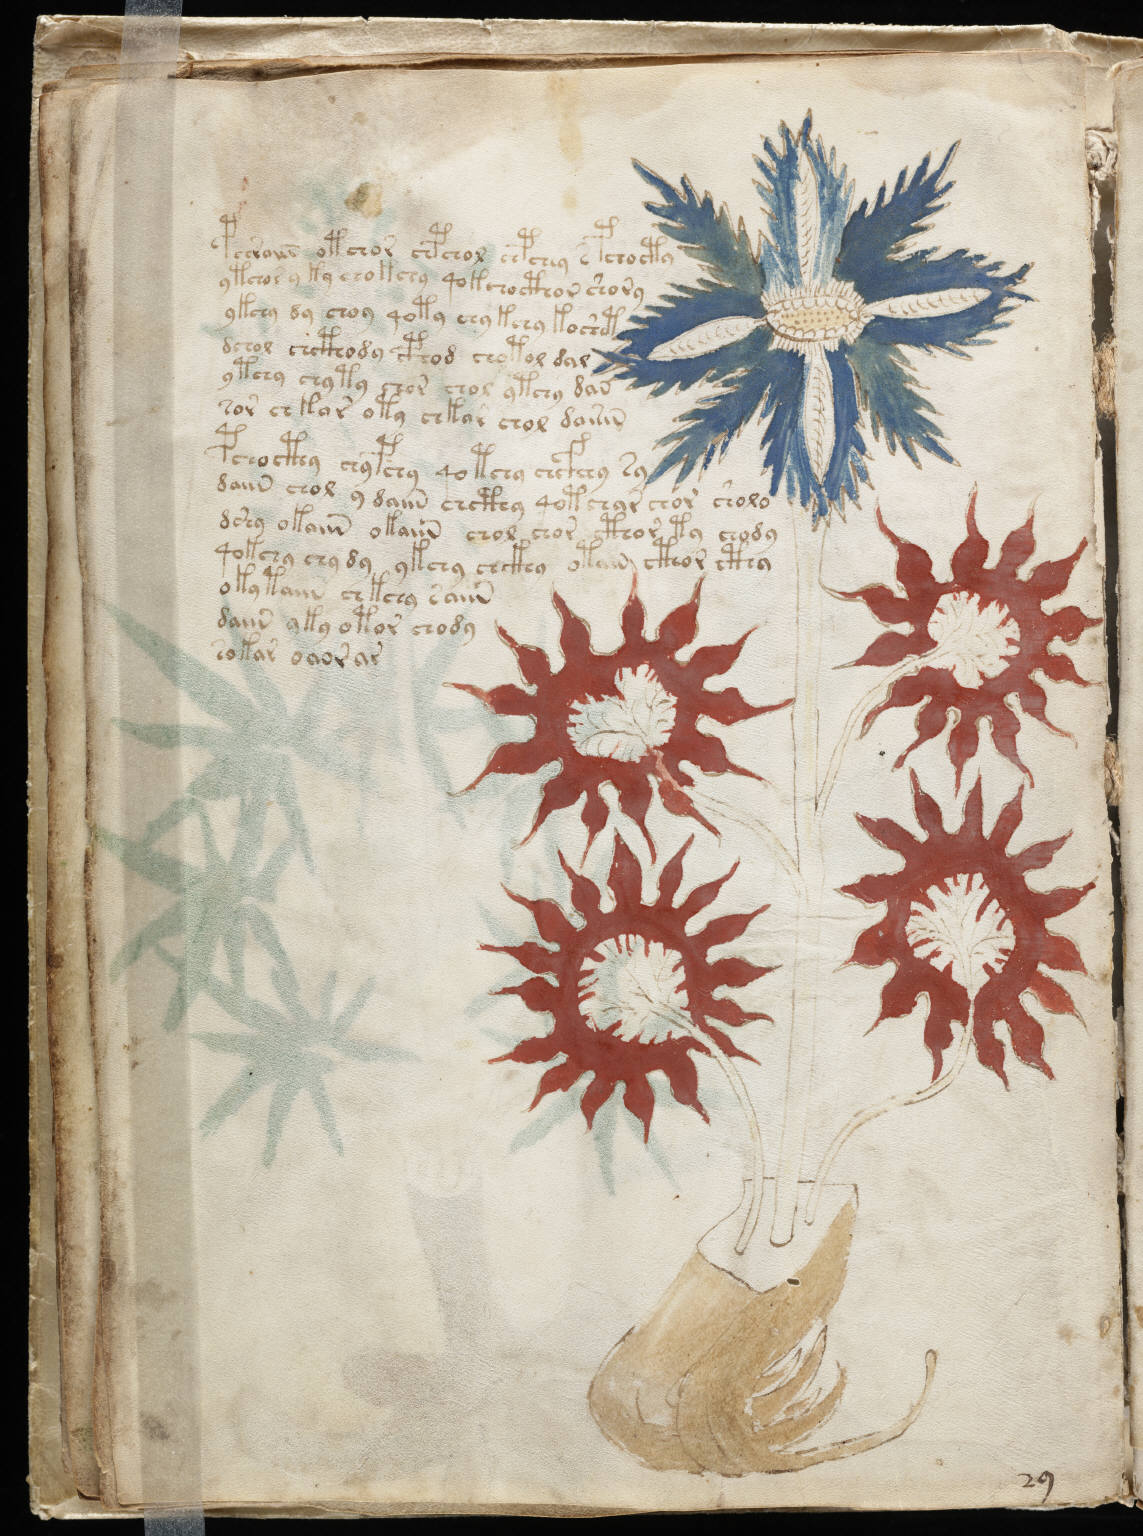
\includegraphics[width=0.5\textwidth]{figures/voynich_32.jpg}
    \caption{A page from the Voynich Manuscript (\url{https://commons.wikimedia.org/wiki/File:Voynich_Manuscript_(32).jpg}, uploaded by user JovanCormac; public domain because the creator has been deceased for over a century).}
    \label{fig:voynich32}
\end{figure}




The manuscript features colorful paintings of plants, stars, and nude
women in pipes (it looks as odd as it sounds). A page is shown in
Figure~\ref{fig:voynich32}. The imagery would suggest that the book
might discuss recipes, potions, astrology, and medicine.  As shown in
Figure~\ref{fig:voynich-text}, the text appears to be written from
left to right without punctuation.  Groups of characters are separated
by spaces, just like words in the Latin alphabet, but it is not clear
whether these groupings can be considered meaningful words.



Researchers have struggled with the Voynich Manuscript for centuries.
Some people have claimed to have deciphered it, but only by telling
stories after the fact.  If the manuscript has a meaning at all, then
it can only be truly deciphered by a specific, reproducible process
for mapping the text to a particular human language and back again.


\begin{figure}[H]
    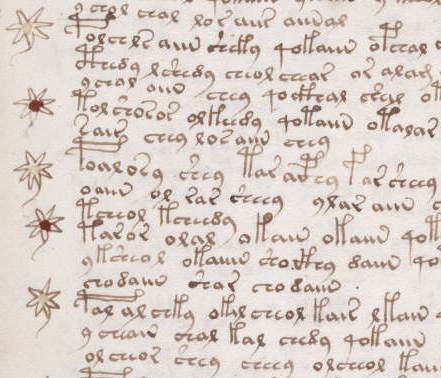
\includegraphics[width=0.5\textwidth]{figures/voynich_recipe107r.jpg}
    \caption{A close-up of some writing in the Voynich Manuscript (\url{https://commons.wikimedia.org/wiki/File:Voynich_manuscript_recipe_example_107r_crop.jpg}, uploaded by user Tomhannen; public domain because the creator has been deceased for over a century).}
    \label{fig:voynich-text}
\end{figure}

One way to make progress on the Voynich Manuscript is to study it as a
historical artifact -- who owned it, who wrote about it in the past,
who would have had access to the materials used to produce it, how it
compares to other historical manuscripts, and so on.  From such
investigations, it appears that the Voynich Manuscript originated in
Europe in the 1400s, perhaps in the Alpine region, although it is
still an open question who produced it and why. As we will see, the
Voynich Manuscript is full of contradictions from every angle: Here,
it is puzzling that the manuscript is physically clearly European
while the content appears alien.

Another way forward is to start from the illustrations, assuming that
some ``word'' (space-separated string) on the page may refer to the
picture -- perhaps one of the first words, one that appears frequently
on that page, or one written near the illustration.  Just as children
learn early words from pointing and naming physical objects, this
strategy would leverage the fact that language refers to entities in
the world.  But without knowing which words to associate with the
picture, it is not easy for this strategy to get off the ground.
Among the illustrations, more contradictions emerge: The paintings use
expensive material but also look slapdash, and the depicted plants are
a mix of real and fantastical.

Most relevant for our purposes here, a third strategy is to explore
the manuscript as a (digitized) text, asking to what extent it
resembles other texts.  This strategy builds on the idea that we can
identify quantitative patterns within text even without reading it or
knowing how it relates to the outside world. That is, techniques
employed to treat text as worthy of research in and of itself can be
used to help decipher the nature of mysterious texts.

There is no Unicode mapping for the unusual handwritten character
system used in the Voynich Manuscript, so in order to digitize the
text, each Voynich character has been mapped to an ASCII version --
involving difficult judgment calls about whether multiple
subtly distinct markings should be grouped as one character or
two. The Voynich writing system uses about 22 different characters,
suggesting that the writing system is an alphabet or an abjad rather
than a syllabary or a logographic system (which require more distinct
characters).
%The digital version of the Voynich Manuscript also includes
%information about the pagination, line breaks and the genre of
%illustrations (separating the sections on stars, plants, and so on).


From the standpoint of textual statistics, we find even more
contradictions.  Just like in text of known languages such as English,
some characters are much more frequent than others, and some tend to
appear in pairs or in certain positions of a word.  A few words appear
very frequently, and many words appear very infrequently (Zipf's power
law; see Section~\ref{sec:zipf}).  A relatively infrequent word may
appear quite frequently on a given page, which occurs in
known-language text with words relevant to a particular topic.  But
unlike text of known languages, there are also characters with a
striking tendency to appear at the beginning or end of a line, which
is highly unusual in prose, where line breaks are generally not
meaningful.  And while text in known languages tends to include highly
frequent bigrams (e.g., \exword{of the}, \exword{it is}), the Voynich
Manuscript surprisingly lacks such predictable bigrams.  Instead, the
same word is often repeated twice or three times in a row, or repeated with a difference of only one character, which is highly unusual.

In other words, the Voynich text does not pattern like text in any
known language, but has enough in common with known-language texts
that it is unlikely to be gibberish. It remains mysterious whether it is a hoax, a cipher, or a meaningful document.  If you explore this
mystery further (which we recommend!), you will learn more about language,
writing, history, and digital humanities.
\end{underthehood} 
\end{tblsfilledsymbol}


\section{Available (English) corpora}

Here are some of examples of English-language corpora that you can explore.  For each one, it is useful to consider who built it and why, and thus what kinds of questions the corpus can help to answer.

\begin{itemize}
\item The million-word Brown Corpus \citep{FrancisKucera:1979} is the earliest machine-readable corpus of American English.  It is a
\keyword{balanced corpus}, meaning that it aims to represent a balance
of different genres -- news, editorials, religious texts, fiction,
magazines, academic articles, and so on.  If you know Python,  you can access this corpus through Python's Natural Language Toolkit \citep{LoperBird:2002}.

\item Project Gutenberg digitizes various books old enough to be
in the public domain.  Some of these texts are available through the
Natural Language Toolkit in Python \citep{LoperBird:2002}.


\item The British National Corpus \citep{BunardAston:1998} comprises one
hundred million words of British English from the late 20th
century.  Ninety percent of the data comes from a balance of different
written sources and ten percent comes from transcribed speech.  The
corpus can be browsed through a web interface, or downloaded in XML
format.

\item CHILDES \citep{MacWhinney:2000} is a suite of corpora offering
transcripts, audio, and video of interactions between children and
their care-givers in several languages.  This corpus, which can be
browsed and downloaded from the CHILDES website, is used to study the
language exposure and development of children.

\item The website \url{English-Corpora.org} houses dozens of different
English corpora, many of them spearheaded by  Mark
Davies.  Most of these corpora can be browsed through a free web
interface, but require a paid license to download all the data.  The
corpora include:

\begin{itemize}
\item The Corpus of Contemporary American English \citep{Davies:2009} -- a billion words from a
balance of both written and spoken genres from 1990 until the present.
This is a \keyword{monitor corpus}, meaning that it is updated each
year.

\item The Corpus of Historical American English \citep{Davies:2012} --
four hundred million words, balanced across genres, from 1810 to the
present.  All texts in this corpus are annotated with dates, allowing
historical comparisons.

\item The Coronavirus Corpus -- comprising media text annotated by
date throughout the  pandemic -- recording the frequency over
time of phrases such as \exword{anti-mask}, \exword{reopen}, and
\exword{social distancing}.
\end{itemize}

\item Social media data (from Reddit, Yelp, Stack Exchange, and so on)
is often already available in a user-friendly format online; search online before you try to scrape such data yourself.  But some such repositories were taken down around 2023 after large language models were trained on them without compensation. 



\end{itemize}

You can explore further publicly available corpora at repositories hosted by Lancaster University (\url{https://cqpweb.lancs.ac.uk/}) and Georgetown University (\url{https://gucorpling.org/cqp/}).  This chapter focuses on text, but there are also audio and video
corpora, which are important, for example, in the study of
pronunciation and the relation of language to embodied action.

As you can guess,
choosing a corpus begins with one's research question.  What data do
you need?  Are you doing \keyword{exploratory research} -- looking for
interesting patterns, getting a sense of the data, trying to generate
hypotheses?  Are you doing \keyword{confirmatory research} -- testing
a falsifiable claim?  What corpus data would verify or falsify that
claim?  What numbers will you collect, what other numbers will you
compare them to, and how will you analyze them statistically?  To what
extent will your findings generalize beyond your particular corpus?

Imagine that you are looking for an extremely low-frequency phenomenon,
such as the bigram \exword{think whether} explored by
\citet{White:2021}. In this case, you might simply use a web search as
a corpus: One can search for a phrase online to see if people use it,
or compare the number of hits for two alternative phrases. The web is
massive, which is good for finding low-frequency phenomena. It may
also, however, contain typos, duplicates, and gibberish, which are
less likely to be found in a curated corpus.

Your research question might also require certain metadata or annotations: Above,  we encountered corpora of sentences annotated for their dependency structure,  requests annotated for their politeness, compound words annotated for the relation between the two
words, and menus from cheap versus expensive restaurants.   Usually, a corpus with such features tends to be smaller than one without.

If you need metadata or annotations that are not already available, you might have to construct the corpus yourself.  How will you gather annotations -- from whom, at what rate of pay,  with what annotation guidelines?  If you gather annotations from multiple people, how do you ensure that they are consistent with one another?  As the researcher, it might be quickest to annotate data yourself, but will your annotations be biased by your hypothesis?  You may have to consider privacy concerns (whose data are you using, and what have these people consented to?) alongside principles of open science, and weigh these factors to decide whether you will make your data available to the community.

% Depending on the research question, you may need your corpus to offer certain \keyword{metadata} -- information about the speaker/writer, their demographic traits, their audience, the date, part-of-speech tags or syntactic dependency parses (which may be built-in to the corpus or added afterward), and so on. 
%If you are working with transcribed speech, were filler words
%(\textit{um, uh}) left out?

% a corpus of tweets about mass shootings,

% If your research question targets a very specific type of text, however, you may need to create a custom corpus; above, 

You will also have to consider how you need to
access the corpus. If you are new to working with data, it may seem
like clicking around on a free web-interface tool is sufficient -- and
for many tasks, it is -- but for some questions, you may need to
write code to process the data yourself.

In choosing or creating a corpus, it is also important to consider how
the corpus may be biased.  How were the data selected?  Whose data does it represent?  Many corpora
favor the standardized form of a language over varieties spoken by
people who have less power.  Our discussion has also been biased
towards English; in general, the more geo-politically powerful a
language is, the more corpora are available in that language.
\keywordAs{Low-resource languages}{low-resource languages} by
definition do not have large corpora, which makes it harder to study
them and to build language technologies for their speakers.  Like any
other data, corpora reproduce the inequalities of the society in which
they were created.


\section{How are words distributed in text?} 

Investigating text as data often involves counting words in the text.
But what are words, how do we count them, and how are words
distributed in text?

A ``word'' may seem obvious to you, but, from a theoretical
standpoint, it is not easy to define.  Should \exword{mother-in-law}
count as one word or three?  What about \exword{flu shot}, mentioned in Section \ref{sec:tokenize}? What about languages such as Chinese,
where bisyllabic ``words'' consist of two meaningful morphemes, each
of which acts word-like itself (similar to the English compound verb
\exword{kickstart})?  But from a practical standpoint, it is simple
enough to define a Latin-alphabet ``word'' as the text between spaces
-- the process of \keyword{word tokenization} mentioned in \chapref{ch:call} (recognizing that tokenization is harder in writing systems that do not use spaces).
Then you have to decide if you want to \keyword{lemmatize} the words
by removing grammatical inflection (e.g., standardizing
\exword{running} and \exword{ran} into basic verb form \exword{run}), or whether you might want to \keyword{stem} the words by removing morphological markers that determine its part-of-speech (standardizing \exword{democracy} and \exword{democratic} into \exword{democra-}).

%\mad{There are two things happening with this example: tokens mapping
%to types and tokens-or-types mapping to lemmas}

Some words are extremely frequent across all English texts (\exword{the,
a, for}), while other words (\exword{horse, dance, stoic}) are
infrequent or vary widely in frequency depending on the particular
text.  These two types of words map onto the distinction proposed in
linguistics between \keyword{function words} and \keyword{content
words}.

Function words (determiners such as \exword{the, a,} and
\exword{every}; prepositions such as \exword{for, to}, and
\exword{with}) are difficult to paraphrase, very rarely  admit 
borrowings or neologisms (thus are said to be a \keyword{closed class}),
and provide information about the grammatical structure of a sentence.
Function words comprise the \keyword{stop words} that are sometimes
filtered out of text on the grounds that they do not make relevant
distinctions between documents.  On the other hand, function words can
be crucial for tasks such as author profiling and author
identification.

Content words (nouns, verbs, adjectives, and adverbs -- \textit{unicorn, run, pretty, slowly}) are much easier
to paraphrase, allow endless borrowings and neologisms such as \exword{quaranteam} (thus, they constitute an
\keyword{open class}), and supply the content of a sentence.  The
boundary between function words and content words is fuzzy -- with
borderline cases such as \exword{have} in \exword{have eaten} or
\exword{take} in \exword{take a shower} -- but the prototypical
examples on each side are clear.

%\mad{Added a bit here to tie back to the original 3 questions} - great thanks!
  Having
introduced these qualitative concepts of what a word is, let us turn
to counting words, and to the principles underlying the quantitative
distribution of words in text.

\subsection{Zipf's laws}
\label{sec:zipf}

The American linguist George Kingsley Zipf (1902-1950;
\citealt{Zipf:1932}) formulated two fundamental observations about
word frequencies: \keyword{Zipf's power law} and \keyword{Zipf's
brevity law} (each of which, confusingly, is sometimes just called
``Zipf's law'').

Zipf's power law observes that the frequency of a word is inversely
proportional to its frequency rank.  To step back, one must first
understand the \keyword{type-token distinction}: A word type is a
unique word, no matter how many times it is repeated, while a word token is a specific usage
of a word, counting all iterations thereof.  For example, \exword{a
rose is a rose is a rose} (a poem fragment by the American modernist
poet Gertrude Stein) contains three word types (\exword{a, rose, is})
and eight word tokens.  The type-token distinction allows us to
explore how various word types differ in their token frequency.

Instantiating Zipf's power law, the first-ranked English word by
frequency in the Brown Corpus is \exword{the}, and this word type
accounts for about six percent of all word tokens.  \textit{The} is about
twice as frequent as the second-ranked word, \textit{of}, which
accounts for about three percent of word tokens.  \textit{The} is roughly three
times as frequent as the third-ranked word, \textit{and}, which
comprises 2.6 percent of tokens.  \textit{The} is about four times as
frequent as the fourth-ranked word, \textit{in}, which comprises 1.8 percent of tokens.  And so on.  This pattern is observed across all texts and languages, for reasons that are still not fully understood.

\begin{figure}[htbp]
  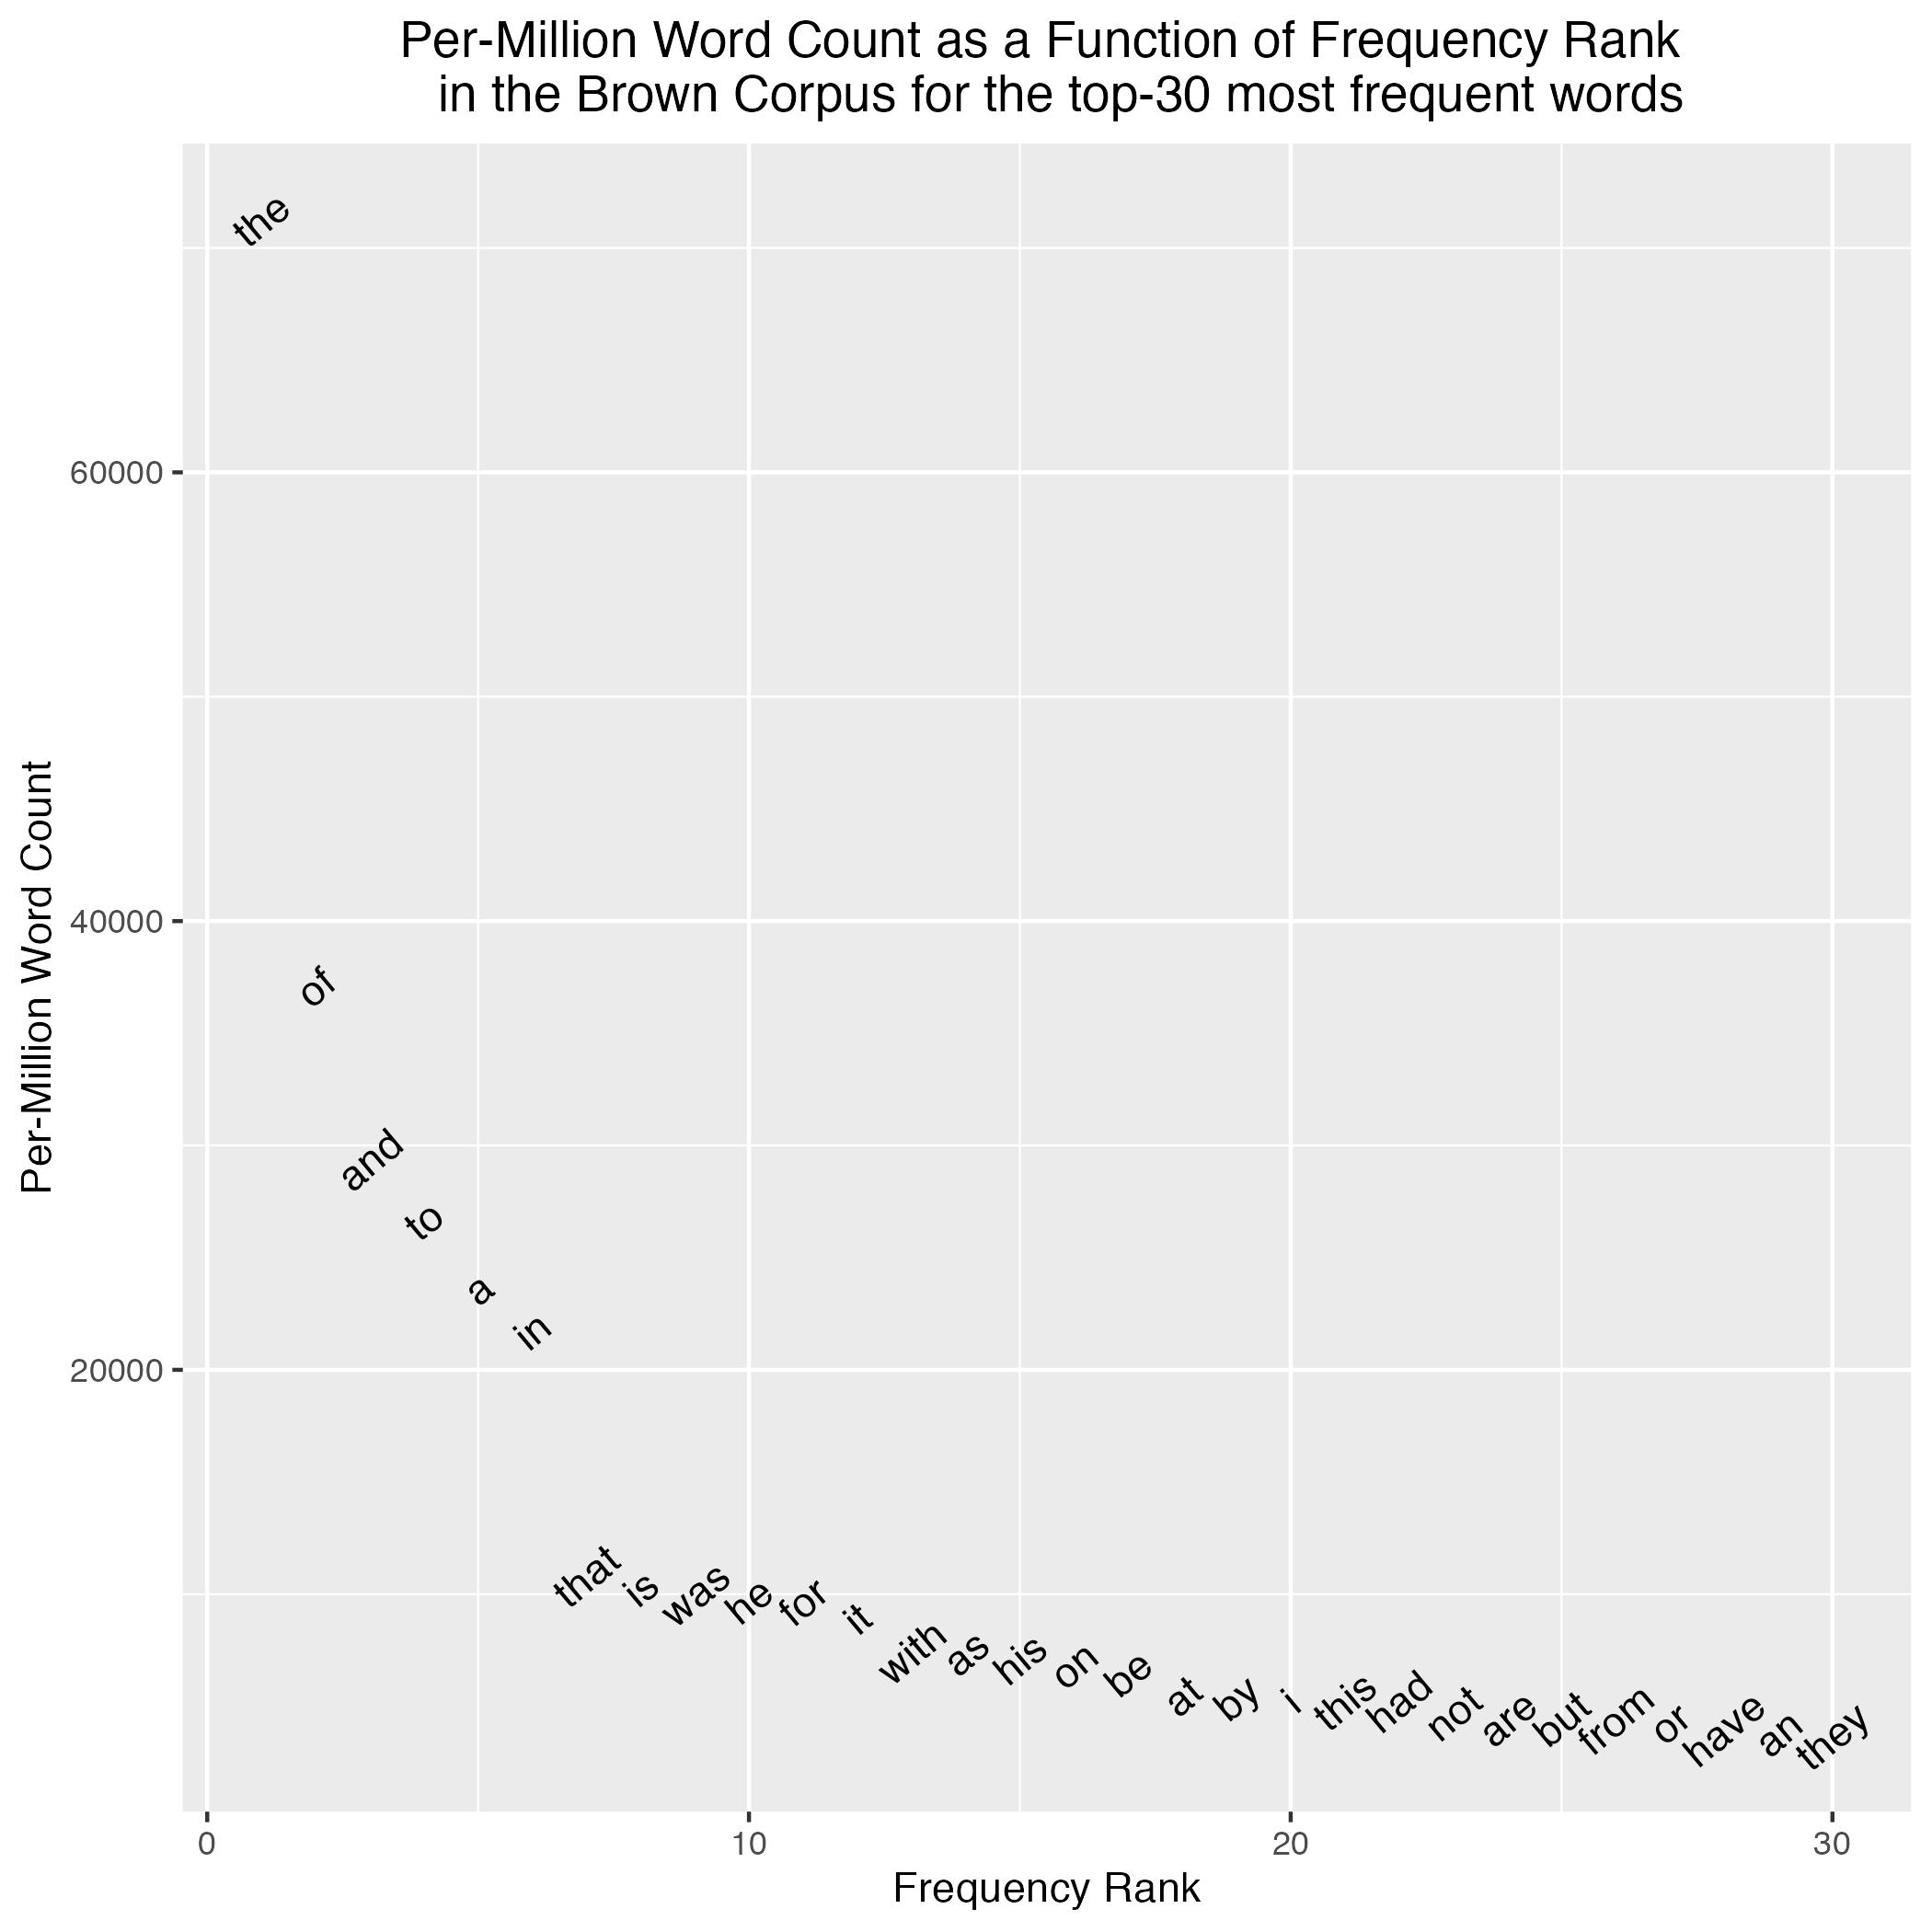
\includegraphics[width=0.8\textwidth]{figures/zipf_power_glass.jpg}
  \caption{Per-million-word frequency of words in the Brown Corpus as a function of their frequency rank (ordered from left to right as the first most frequent word, the second most frequent, and so on).}
  \label{fig:zipfpower}
  \end{figure}
  
When we plot a word's frequency rank on the $x$-axis and its frequency
on the $y$-axis (\figref{fig:zipfpower}), we observe that the frequency of words falls steeply
from the top few very frequent (function) words to the \keyword{long
tail} of very many infrequent (content) words.  This graph represents
a \keyword{power law distribution}, generated by a mathematical
function where $y$ is a function of $x$ raised to some power $\alpha$
(usually, a negative value). 

While first observed in the domain of words, Zipf's power law extends
to many other phenomena.  The distribution of wealth, social media
followers, citations of articles, the populations of cities, the
number of workers at companies, and other phenomena involving the
unequal distribution of scarce resources follow a similar pattern: A
few individuals have an enormous amount (of wealth, followers,
citations, population, workers, etc.), and most have very little.

In contrast, other phenomena follow the familiar \keyword{normal
distribution}: Most people are of about average height/weight, with a
few very small and very large people at the edges of a \keyword{bell
curve}.  The lengths of words, in characters, roughly follow a bell
curve, albeit an asymmetrical one, with a defined lower bound of one
character and an upper bound which is unlimited in principle, given
that new words are created all the time and can be lengthened by
adding productive morphemes such as \exword{un-, anti-}, or
\exword{-able}.  In reality, most English words are between four and
ten characters, with a few very short and very long words at the edges
of the curve, as in Figure~\ref{fig:wordlength}.

\begin{figure}[htbp]
\centering
  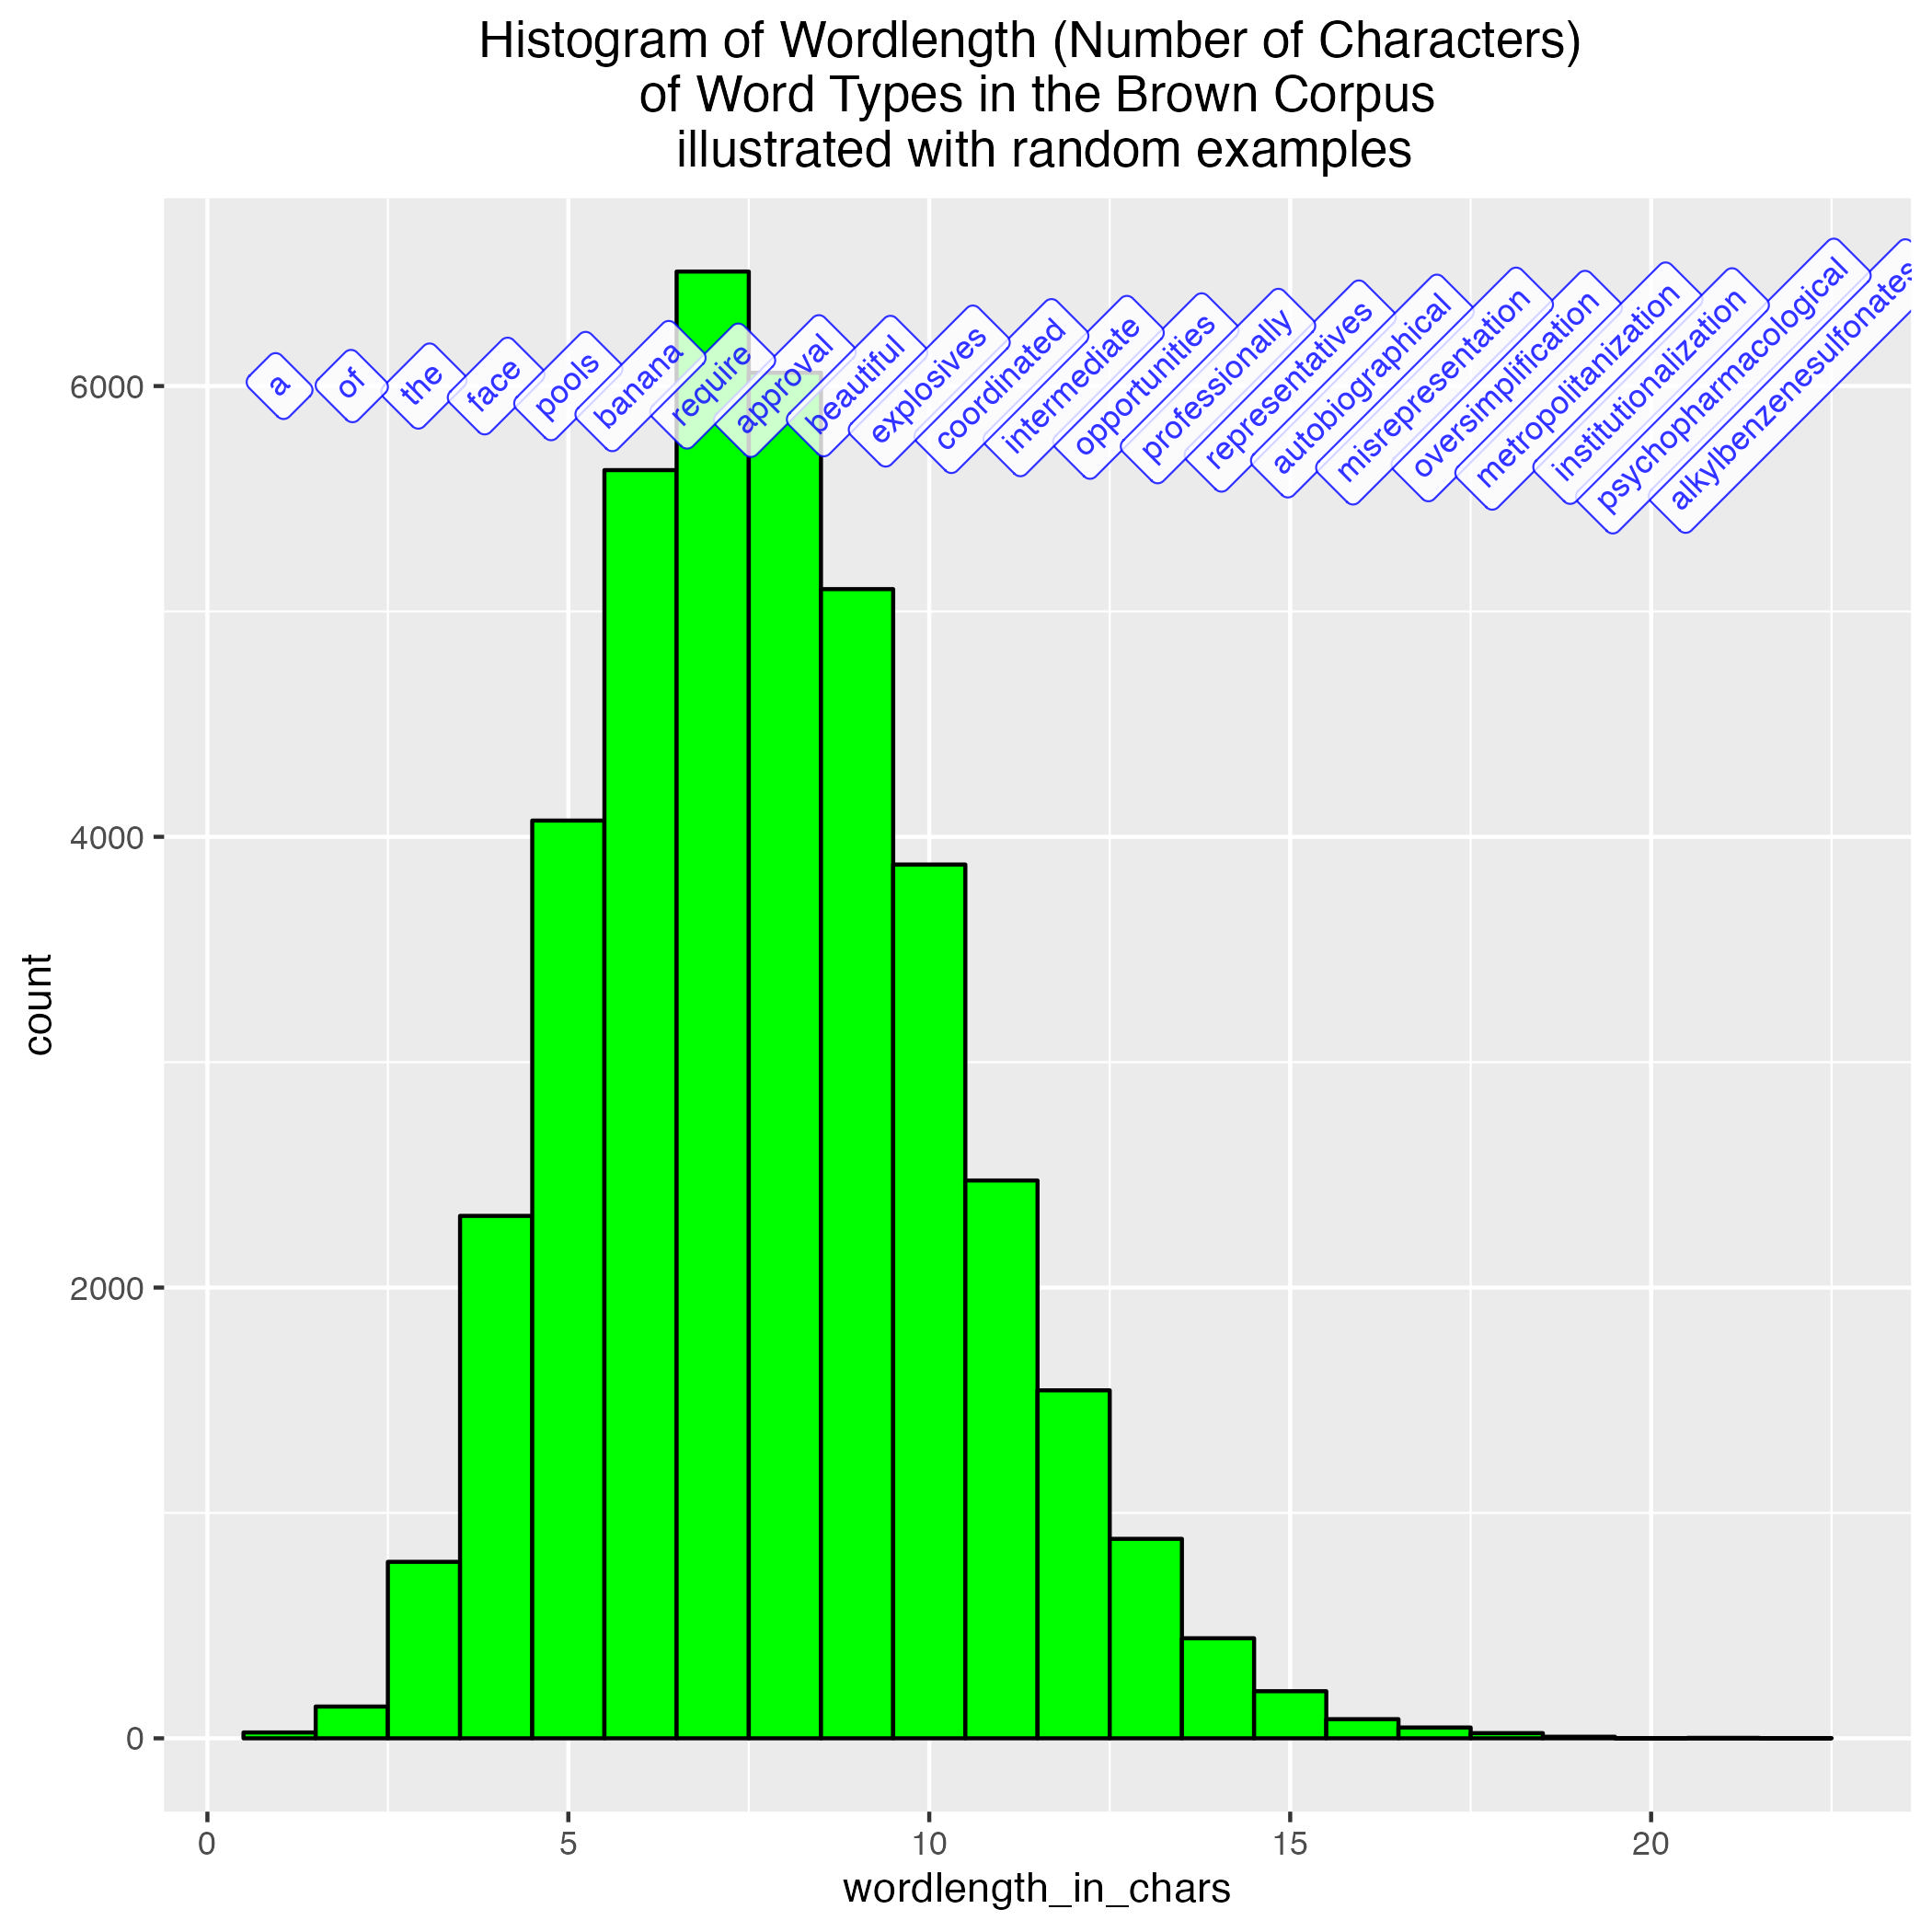
\includegraphics[width=.8\textwidth]{figures/wordlength_hist_glass.jpg}
  \caption{Histogram of the length (number of characters) of all word types in the Brown Corpus.}
  \label{fig:wordlength}
  \end{figure}
  
As a consequence of Zipf's power law, a few word types represent a
plurality of word tokens, and many word types appear once or never in
a given text, as can be seen by the trailing long tail in
Figure~\ref{fig:zipfpower}.  \keyword{Heap's Law} \citep{Heaps:1978} predicts the number
of distinct word types appearing at least once in a document as a
function of its length: That is, the longer the document, the more word
types it will contain, but, as a document gets longer, the marginal
likelihood of encountering a new word type diminishes.  Researchers
use techniques such as \keyword{Laplace (add-one) smoothing} --
pretending you have seen a word type once rather than zero times, to
avoid dividing by zero in various equations -- to account for the
reality that any NLP technique will encounter
new word types in new data.  A \keyword{hapax legomenon} (`said once' in Greek) is a word that occurs only once in a document.  About 38 percent of words in the Brown Corpus (such as \exword{mirthless} and \exword{pastels}) are \exword{hapax legomena}, and another 14 percent are \exword{dis legomena} (such as \exword{syndicated} and \exword{lamentations}), occurring only twice. 
% updated from my own Brown corpus data, Summer 2023 - LG

The second of Zipf's laws, Zipf's brevity law, observes that across
all languages and texts, more frequent words tend to be shorter (in
characters or syllables) than less frequent words. Figure
\ref{fig:zipfbrevity} shows that the shortest
words are most frequent, while longer words are less frequent. For
example, the top ten most frequent words in the Brown Corpus
(\exword{the, of, and, a, in, to, is, was, I, for}) are all one
syllable, three letters or less -- lower than the most common length
of four to ten characters -- while the hapax legomena
(\exword{mirthless, pastels}) are longer.  The precise mechanisms
are debated, but intuitively Zipf's brevity law suggests that
languages evolve for efficiency: When the most frequent words are
short, communication takes less effort.  Imagine how onerous it would
be if the meanings for the words \exword{the} and \exword{therefore}
were swapped!

\begin{figure}[htbp]
\centering
  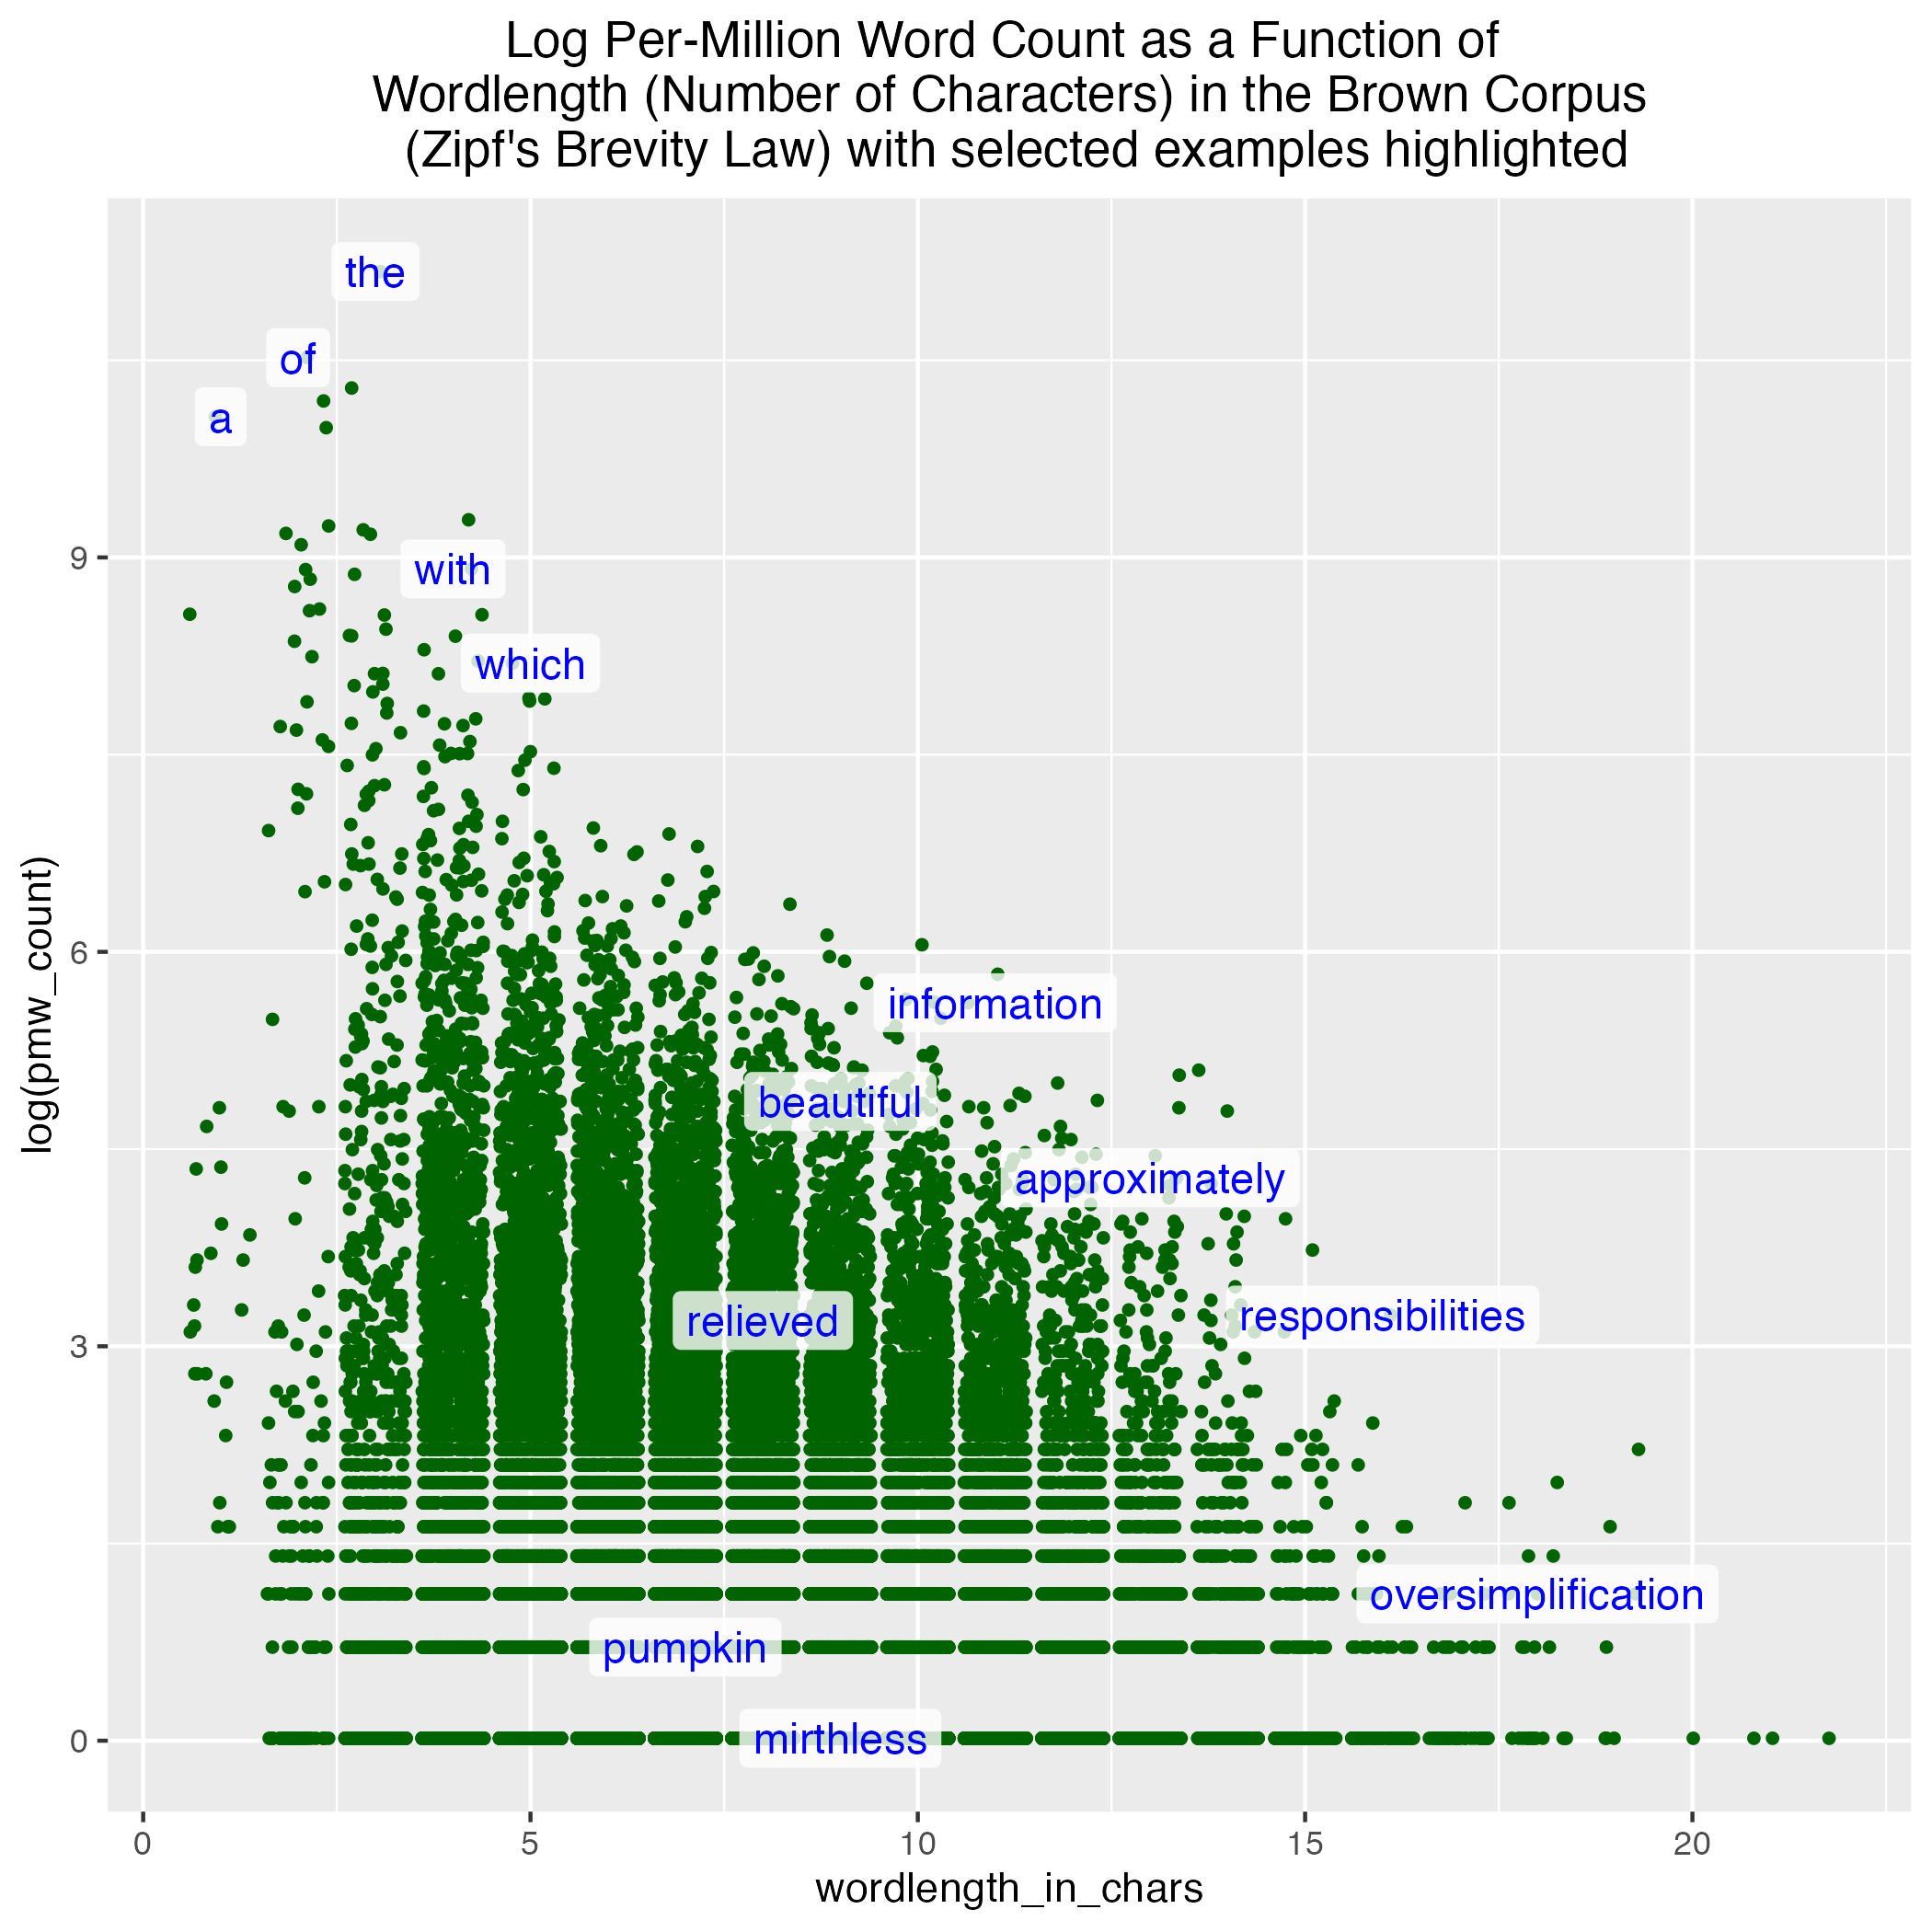
\includegraphics[width=.6\textwidth,clip,trim=0 10 10 0]{figures/zipf_brevity_glass.jpg}
  \caption{Log per-million-word frequency of English words in the Brown Corpus as a function of their length in characters.}
  \label{fig:zipfbrevity}
  \end{figure}


\subsection{Topic models}

So far, we have considered the distribution of words at a large scale.
But how are words distributed across smaller documents, such as
individual paragraphs, chapters, articles, tweets, or product reviews?
Documents can differ by \keyword{genre} (e.g., personal anecdotes
versus news articles versus fiction) and by \keyword{topic} (e.g.,
text about pets versus politics versus travel); of course, there
is some interaction between genre and topic, as different genres favor
different topics. Crucially, texts about different topics are likely
to differ in the distribution of content words: A text about animals will contain words like \exword{cat,
dog,} and \exword{fish}, while a text about politics will mention
words like \exword{election, poll,} and \exword{candidate}.

\keywordAs{Topic modeling}{topic modeling} is a technique used to discover how different
documents and words reflect these different topics.  A topic, on this view, is a probability distribution
of words associated with that topic: In the ``pets'' topic, for
instance, the words \exword{cat} and \exword{dog} are quite likely to appear.
A document is also a probability distribution over the topics
that it discusses, as conveyed by the words therein and the topics
that they evoke.  A tweet about dogs and cats is most probably
associated with the topic of pets, less probably associated with
politics.

Topic modeling is generally used as an exploratory technique when you
have a lot of documents, with no topic labels assigned to them at the
outset, and you do not know in advance which different topics they
discuss.  For example, maybe you are an attorney reviewing a thousand
emails turned over as part of a court proceeding, looking for emails
about a particular project which may have involved fraud.  Instead of
reading all the emails by hand, you might use topic modeling to
cluster the emails into different topics (office-wide announcements,
hiring, projects) to get a bird's-eye view of the data before you dive
in, and to target your attention to emails discussing the most
relevant topics.   As for other applications, perhaps you have surveyed customers asking them
for open-ended feedback about your product, and you want to gauge the
different topics discussed; or perhaps you want to show users more social media posts about the topics that seem to interest them.

One of the classic topic modeling techniques is called \keyword{Latent
Dirichlet Allocation}, LDA for short \citep{Blei-etal:2003}.  \exword{Latent} (which means
`hidden') refers to the idea that a document's topic, in many cases,
is implicitly inferred rather than explicitly labeled.
\exword{Dirichlet}, named after a German mathematician, is a type of
probability distribution; as we'll see, the idea is to associate: (i)
each topic with a probability distribution over the words associated
with it, and (ii) each document with a probability distribution over
the topics it discusses.  \exword{Allocation} refers to the fact that
we allocate each word and each document to the topic(s) most strongly
associated with it.  LDA is a type of
\keyword{unsupervised learning}, because we never provide any labels
or ``right answers'' for the algorithm to generalize; instead we just
give it some data and ask it to find the meaningful topic groupings
therein. We will see more examples of both supervised and  unsupervised learning in
Chapter~\ref{ch:text-classification}.

LDA works as follows: We begin with a set of documents -- for example,
emails turned over during legal proceedings.  Next, we choose the
number of topics we want to find. When you are using topic modeling
for exploratory purposes, it is common to try different numbers of
topics, settling on the one that yields the most intuitive results;
for our purposes, let us imagine that we want two topics. Then we
randomly assign every word token in every document to one of those
topics.  With two topics, we essentially assign each word token to a
topic by a coin flip.  As is common in topic modeling, we lemmatize
all words and filter out stop words.

Next, we build a matrix, as in Table~\ref{tab:topic-modeling1}, where
the rows are word types, the columns are topics, and the values are
the number of tokens of that word type assigned to that topic.  The
columns (topics) are labeled with numerals; any descriptive label
(\exword{pets, politics}, etc) must be provided by a human who
interprets the output of the topic model once it is complete.

\begin{table}
\begin{tabular}{llr}
\lsptoprule
& Topic1 & Topic2 \\ \midrule
dog & \textbf{5} & \textbf{4} \\
cat & 8 & 7 \\ 
election & 7  & 8 \\ 
candidate & 2 & 4  \\
walk & 5 & 5 \\ 
weekend & 10 & 14 \\ 
pet & 2 & 3 \\ 
\lspbottomrule
\end{tabular}
\caption{Topic modeling with two topics, stage one: Random assignment of words to topics.}
\label{tab:topic-modeling1}
\end{table}



After we have gone through this process of assigning words to topics at
random, we iterate through each word token in each document, meaning
that we just look at each word individually rather than any grammatical or semantic relations
between them.  Each word token has already been assigned a topic by a
coin flip, represented by the parenthetical numbers in \REF{ex:dogdoc}.

\ea  \label{ex:dogdoc} dog(2) walk(1) weekend(2) pet(1)
\z

We begin with the token \exword{dog} in \REF{ex:dogdoc}.  This token of
\exword{dog} has previously been randomly assigned to Topic 2; we
now un-assign the topic of this word token.  We update our
term-by-topic matrix to reflect this change (decrementing the first row,
second column of our matrix to 3 instead of 4).  Next, we re-assign a
topic to this token of \exword{dog} token by considering two factors:
(i) the topics most prevalent in this particular document; and (ii)
the topics most commonly associated with the particular word type
\exword{dog}.  To quantify the topics most prevalent in this document,
we observe that two of the remaining three words (\exword{walk} and
\exword{pet}) have been assigned to Topic 1, so Topic 1 is twice as
prevalent in this document as Topic 2.  To quantify the topics most
commonly associated with \exword{dog}, we observe that \exword{dog} is
used five times in Topic 1 and three times in Topic 2 (which we read from the
first row of our matrix, with the 4 decremented to a 3, as we have
un-assigned the topic of the current token of \exword{dog}).  Both
this document and the word type \exword{dog} favor the assignment of
Topic 1 to this token of \exword{dog}.  So we update the assignment of
\exword{dog}, and update our term-by-topic matrix, as in
Table~\ref{tab:topic-modeling2}.

\begin{table}
\begin{tabular}{llr}
\lsptoprule
  & Topic1 & Topic2 \\ \midrule
  dog & \textbf{6} & \textbf{3} \\
cat & 8 & 7 \\ 
election & 7  & 8 \\ 
candidate & 2 & 4  \\
walk & 5 & 5 \\ 
weekend & 10 & 14 \\ 
pet & 2 & 3 \\ 
\lspbottomrule
\end{tabular}
\caption{Topic modeling with two topics, stage two: New values based on data-driven reassignments.}
\label{tab:topic-modeling2}
\end{table}


\ea  dog(1) walk(1) weekend(2) pet(1)
\z

We keep going through each word token in each document, and then go
through it all again as many times as we want (perhaps 50 or 100
times).  Eventually, the words that tend to co-occur within the same
document will end up being assigned to the same topic, perhaps
something like in Table~\ref{tab:topic-modeling3}.

\begin{table}
\begin{tabular}{llr}
\lsptoprule
& Topic 1 & Topic 2 \\ \midrule
dog & 9 & 0 \\
cat & 14 & 1 \\ 
election & 1  & 14 \\ 
candidate & 0 & 6  \\
walk & 8 & 2 \\ 
weekend & 12 & 12 \\ 
pet & 5 & 0 \\ 
\lspbottomrule
\end{tabular}
\caption{Topic modeling with two topics, final stage: Final numbers after some set number of iterations.}
\label{tab:topic-modeling3}
\end{table}

The output of the topic modeling yields, for each document, a
distribution of the topics most strongly associated with it; and for
each topic, a distribution of the words most strongly associated with
it.  Then you have to look at each topic and its associated words, and
decide if these words (\exword{cat, dog, pet}) indeed evoke a cohesive
theme.  You can use your own human judgment to give a name to each
topic. In our  toy example, Topic 1 involves pets.

While it is important to understand how topic modeling words under the
hood, in real life you will probably use one of the many libraries (in
Python or R) which does it for you.  You might also use a fancier
version of topic modeling that leverages richer information about
which words are similar to one another, in ways to be explored later
in this chapter.

Because topic modeling is a way of exploring your data, you may want
to try it several different times for a fuller exploration. You can try different numbers of topics; in general, the more
documents you have, and the more diverse you expect them to be, the
more topics you will need. In addition to lemmatizing words and
filtering stop-words, you can also focus on only certain parts of
speech -- perhaps only nouns, or only nouns and adjectives.  You know
you have succeeded when the topics make intuitive sense, and when the
topic modeling procedure has given you a landscape view of the data.

More broadly, topic modeling illustrates that you can learn a lot
about words and documents simply by counting which words appear in
which documents.  This general idea underlies a great deal of NLP.

\section{Word meanings as vectors}

In our exploration of topic models, we have used a matrix of numbers
to represent information about different topics and the words that are
associated with them.  We have also represented a sentence as a list
of numerals (a vector) reflecting the topics associated with each word.  In this book and in the study of NLP more
generally, we will keep coming back to the idea of representing
language (topics, words, sentences, documents, etc.) through vectors
and matrices of numbers.  We illustrate with the key idea of
representing a word as a vector that represents some information about
its meaning.

To start off, what is the meaning of a word? The
philosopher of language David Lewis \citep{Lewis:1972} suggests that the way to define
meaning is to focus on what meaning allows you to do.  When you know
the meaning of a word, you can identify the thing, event, or idea that
it refers to; for example, you can point to the furry animals denoted
by \exword{dog}.  You can use the word in a sentence (\exword{I have a
dog}), and reason logically about the sentences in which it is used;
you know that \exword{I have a dog} entails \exword{I have a pet}.
You can identify its synonyms and antonyms (\exword{dog} does not really have clear synonyms or antonyms; but in the realm of adjectives,
\exword{pleasant} and \exword{nice} are roughly synonyms to each
other, and antonymous with \exword{unpleasant}).  You also know the
word's \keyword{hypernyms} (more general words -- \exword{animal} is a
hypernym of \exword{dog}) and \keyword{hyponyms} (more specific words:
\exword{poodle} is a hyponym of \exword{dog}).  You can provide other
words (\exword{cat, bark, walk}) that fit into the same
conceptual domain.  If you know the meaning of a word that describes a
relationship or a transaction, you know which other words describe
alternate perspectives on the same relation: You know how
\exword{parent} relates to \exword{child} and how \exword{buy} relates
to \exword{sell}.  You can also identify the formality level and
emotional sentiment associated with the word: You know that
\exword{doggie} is informal and that \exword{win} feels positive.  In
other words, knowing the meaning of a word means knowing how it
relates to other words.

For a computer, however, the string of characters \exword{dog}
reflects none of that information.  Of course, a computer could look
up \exword{dog} in a dictionary, but the dictionary would provide a
prose definition which is just a longer string of characters.

The problem is that to a computer, text is \keyword{categorical}: A
string of characters is just a string of characters, with no
organizing principle relating it to any other string of characters or
any other information.  Humans can interpret text by imagining the real-world situation that it describes, but such mental representations and real-world situations are not legible
to a computer.  Moreover, the idea of edit distance from Chapter
\ref{ch:writers-aids} quantifies the difference in spelling between
one word and another, but -- given that an alphabetic writing system
represents sound only -- captures nothing about meaning.

In contrast to text, numbers are \keyword{continuous}, meaning that
they can be organized on a number line (or, for a vector of numbers,
plotted in a coordinate space) in ways that represent meaningful
relations between them.  While there is no way to carry out
mathematical operations on strings of characters, numbers and vectors
can be added and multiplied in ways that capture meaningful
information.  To a human, it is hard to hold too many numbers in one's
mind at once, and a number is not meaningful unless it refers to
something.  But computers are designed to process large quantities of
numbers, and without any representation of the outside world, the
relations between numbers provide valuable information.

In other words, a computer could get more information out of text --
and even ``reason'' about the relations between texts -- if it were
represented as vectors of numbers rather than strings of characters.
But how can a word like \exword{dog} be turned into a numerical
representation?

Actually, even before ASCII was invented in 1963, numerical
representations had been proposed for certain words.  In the domain of
(words for) colors, theorists of vision proposed in the 1800s to
represent each color as a three-valued vector denoting the strength
(out of a maximum of 255) of red, green, and blue light that it uses.
For example, red is denoted as (255, 0, 0), meaning that it is
maximally red and contains no green or blue. 

As shown in Table~\ref{tab:color-words-rgb}, purple is (128, 0, 128), meaning that
it uses equal amounts of red and blue light, but no green.  By using
vectors like (255, 0, 0) and (128, 0, 128) rather than character
strings like \exword{red} and \exword{purple}, we can capture
quantitative relations and operations: For example, the fact that the
color violet (127, 0, 255) is closer to purple (128, 0, 128) than to
red (255, 0, 0); and the fact that red (255, 0, 0) plus green (0, 255,
0) yields yellow (255, 255, 0).  Of course, the RGB color scheme only
applies to color words, but within that realm it transforms
categorical text into meaningful continuous quantities.

\begin{table}
\begin{tabular}{l  l  l  l  l }
\lsptoprule
    color & word &  R &  G & B  \\ \midrule
\cellcolor{red}  & red & 255 & 0 & 0 \\
\cellcolor{yellow} & yellow &  255 & 255 & 0 \\
\cellcolor{green}  & green &  0 & 255 & 0 \\
\cellcolor{purple}  & purple & 128 & 0 & 128 \\
\cellcolor{violet}  & violet & 127 & 0 & 255 \\
\lspbottomrule
\end{tabular}
\caption{Color words represented as three-valued RGB vectors.}
\label{tab:color-words-rgb}
\end{table}

Converging from a different perspective on the same key insight, a
line of work spearheaded by the psychologist Charles Osgood
\citep{Osgood-etal:1957} proposes to capture the emotional meaning of
a word as a three-valued vector denoting human annotations, gathered
from experimental participants, of the word's valence (positive versus
negative), arousal (high versus low energy), and dominance (high
versus low human control).  Using data from \citet{Mohammad:2018} in
which each rating ranges from 0 to 1, \exword{win} is represented as
(0.9, 0.7, 0.8), meaning that it is positive, high-arousal, and
high-dominance, as shown in Table~\ref{tab:vad}.  

\begin{table}
\begin{tabular}{l  l  l  l }
\lsptoprule
    & valence & arousal & dominance  \\ \midrule
\exword{win} & 0.9 & 0.7 & 0.8 \\
\exword{compete} & 0.6 & 0.7 & 0.8 \\ 
\exword{lose} & 0.1 & 0.5 & 0.2 \\
\lspbottomrule
\end{tabular}
\caption{Values for valence, arousal, and dominance.}
\label{tab:vad}
\end{table}

The word \exword{lose} is
(0.1, 0.5, 0.2) -- negative, medium-arousal, and low-dominance, while
\exword{compete} is (0.6, 0.7, 0.8) -- somewhat positive,
high-arousal, and high-dominance.  Again, these numbers capture
important commonalities between words: On an emotional level,
\exword{win} is more similar to \exword{compete} than to
\exword{lose}, sharing high values along the same dimensions.  These
vectors represent only emotional dimensions of meaning, without
capturing any information about the events that they describe.  The
lexicon is transformed into quantities that can be plotted on a
three-dimensional plane.

In each system, the vectors have a length of three, which is about the
maximum vector length that humans can keep in mind and represent
visually on a three-dimensional plane.  But
a computer can handle vectors of essentially any size, so what further
information can be captured that way?  Moreover, the RGB system is
limited to colors and the emotion-vector system is limited to the
words and meaning dimensions that have been laboriously annotated by
humans.  How could these systems be expanded to cover all words, ideally using
information that already lies within text?

The answer is inspired by a famous claim from the corpus linguist
J.R. Firth \citep{Firth:1957} that ``You shall know a word by the company it keeps''.  In
corpus linguistics, the ``company'' that a word keeps consists of its
\keyword{collocations} -- the other words that appear near it in a
corpus.  In Table~\ref{tab:collocation-contexts}, you can see some
examples (adapted, with a few modifications, from 2014 comments on the
web forum AskReddit, gathered by \citealt{Baumgartner-etal:2020}) of
collocational contexts -- here, within a window of five words to the
left and to the right -- for \exword{dog, cat,} and \exword{election}.

\begin{table}
\small
\begin{tabular}{rcl}
\lsptoprule
Left context &  Word & Right context \\ \midrule
friends are pretty annoying. Their  & \emph{dog} & is cute though. (END) \\
cute when it's a small & \emph{dog.} & Also people who encourage their  \\
dog meat industry. You American & \emph{dog} & lovers would be heart sickened  \\  \midrule 
loneliness. Usually, a good cute & \emph{cat} & pic can cheer me up \\
on with me the cute & \emph{cat} & pictures. I almost never browse  \\
but if you've got a & \emph{cat} & that's an asshole I don't \\ \midrule
 elected in a South American & \emph{election} & is testament to that. It \\
and talk about the American & \emph{election} & because I have trouble imagining  \\
kid, they had a family & \emph{election} & on what toy got to \\  
%is being sworn in as & \textbf{president} & standing next to a distraught \\
%another. Remember in The American & \textbf{president} & when Michael Douglass has to \\
%When I'm elected student body & \textbf{president} & I promise to put a \\
\lspbottomrule
\end{tabular}
\caption{Collocation contexts for \exword{dog}, \exword{cat}, and \exword{election} in AskReddit.}
\label{tab:collocation-contexts}
\end{table}

We can turn these data into a \keyword{word-context matrix} where the
entry at row \exword{i}, column \exword{j} records the number of times
that word \exword{i} appears in a context that includes \exword{j}.
As shown in Table~\ref{tab:word-context-matrix}, for example, the top
left corner of this matrix (the \exword{cute} row, \exword{dog}
column) represents the fact that in our tiny data snippet, the word
\exword{dog} appears near \exword{cute} twice.  The \exword{cute} row,
\exword{cat} column reflects that \exword{cat} appears near
\exword{cute} twice; and so on.

\begin{table}
\begin{tabular}{l  l  l  l  l}
\lsptoprule
    & dog & cat & election  & (\ldots) \\ \midrule
cute & 2 & 2 & 0 & (\ldots) \\
American & 1 & 0 & 2  & (\ldots) \\
\lspbottomrule
\end{tabular}
\caption{A small word-context matrix.}
\label{tab:word-context-matrix}
\end{table}

In reality, this matrix would be massive, with as many rows and
columns as there are words in our vocabulary. Because such massive
vectors can be unwieldy even for a computer, there are ways to
compress the information in the word-context matrix so that it is
smaller than the size of the vocabulary, yielding vectors of a few
hundred elements rather than thousands.  

For example, \keyword{Word2Vec} \citep{Mikolov-etal:2013} does not just build word-context matrices like  \tabref{tab:word-context-matrix}, but instead generates vectors by trying to guess the target word from its collocational context, or -- as an alternative way of setting things up -- trying to guess the collocation context from the target word.  Another method, \keyword{GloVe} (short for Global Vectors; \citealt{Pennington-etal:2014}), distills the word's ``global'' distribution in the word-context matrix as in Table  \ref{tab:word-context-matrix} by generating vectors that aim to capture the probability of two words occurring as neighbors to one another.  Both Word2Vec and GloVe yield vectors of a few hundred elements rather than thousands.  Rather than using these tools to build new vectors on a given corpus, you can also download vectors that researchers have already built on massive corpora.  These packaged vectors are known as \keyword{pre-trained} because you do not have to build (train) them yourself.


The important point is that we now have a mathematical implementation
of Firth's idea that we can ``know a word by the company it keeps''.
Each word is represented as a vector (the vector of its row or column)
which captures information about its meaning.  These vectors are
called \keyword{word vectors} or \keyword{word embeddings}, because
they reflect how a word is embedded into its collocation contexts.

Our word vectors capture the intuition that \exword{dog} is more
similar to \exword{cat} than to \exword{election}, as evidenced by the
fact that \exword{dog} and \exword{cat} both are used near
\exword{cute} while \exword{election} is not.  We will learn how to
calculate the similarity between two vectors mathematically in Chapter
\ref{ch:searching}, but for now we can capture the same information
visually by plotting \exword{dog}, \exword{cat}, and \exword{election}
as vectors on a plane where the $x$-axis represents the number of times
the word occurs near \exword{American} and the $y$-axis represents the
number of times it occurs near \exword{cute} (Figure~\ref{fig:word-vectors}), Here, we see that the vectors for
\exword{dog} and \exword{cat} are closer to each other on this plane
than the vector for \exword{election}.  Leveraging the mathematical operations that quantitative vectors enable, we can even do addition and subtraction, so that the word with the closest vector representation to the output of \exword{king} - \exword{man} + \exword{woman} is \exword{queen} \citep{Mikolov-etal:2013b}!  


\begin{figure}[htbp]
\small%XXX FIGURE NEEDS TO BE FIXED -- SEE TEX CODE FOR COMMENT XXX
\begin{tikzpicture}[
            > = Straight Barb,
phasor/.style = {thick,-{Stealth}, blue},
angles/.style = {draw, <->, angle eccentricity=1,
                 right, angle radius=7mm}
                        ]
\draw[thin,gray!40] (0,0) grid (4,4);
% coordinates
    \draw[->] (0,0) -- (3,0) coordinate (x) node[below] {\exword{American}};
    \draw[->] (0,0) -- (0,3) node[below left] (y) {\exword{cute}};
% phasors
        \draw[phasor] (0,0) -> (1,2) coordinate (i)  node[right] {\exword{dog}};
        \draw[phasor] (0,0) -> (0,2) coordinate (i)  node[right] {\exword{cat}};
        \draw[phasor] (0,0) -> (2,0) coordinate (i) node[below left] {\exword{election}};
% angles drawn by pic
\coordinate (X)   at (0,0);
% XXX fix the following line:
% \draw pic["$\phi$",angles] {angle=x--X--v};
\coordinate (X)   at (1,1);
% XXX fix the following line:
% \draw  pic["$\theta=\phi-\SI{90}{\degree}$",angles] [right] {angle=i--X--x};
\end{tikzpicture}
\caption{Illustration of word vectors in two-dimensional space.}
\label{fig:word-vectors}
\end{figure}

You may already see a problem here, though: By capturing \emph{the} meaning of a word through its collocations, this framework assumes that a word has \emph{one} single meaning.  But some words have more than one meaning.  The word \exword{mouse} can refer to a rodent or a pointer on a computer -- each with distinct collocation patterns (using data from Reddit):

\ea One night my housemate and I found a dying \emph{mouse} on the floor.

\ex The sophomore dorm had a \emph{mouse} problem, and one student caught one in his trash can and kept it as a pet for about a week.


\ex things change size and move around while you move the \emph{mouse} pointer over them, and they do so at inconsistent speeds.

\ex That's absolutely true but there is a PC mod for it or something that allows you to use a \emph{mouse} and play it like a real first person shooter.

\z

When it describes a  house pest, \exword{mouse} appears in contexts discussing housing situations.  When it describes a digital pointer, it appears in contexts discussing computers and as the direct object of verbs like \exword{move} and \exword{use}.  Still other uses of the word \exword{mouse} might involve the Disney character of Mickey Mouse.  Rather than considering \exword{mouse} to have a single meaning captured by all its collocations, it is more accurate to see it as having several different meanings, each with its own collocations.  Therefore, instead of generating a single vector for each word type, modern techniques will often generate a \keyword{contextual vector representation}, meant to capture the meaning of the word token in context rather than the word type overall.  We will learn more about such tools in \chapref{ch:text-classification}.

Before we get to these refinements, let us consider the power of the ideas we have seen so far.   We have transformed text into a quantitative
representation legible to a computer.  These representations not only
capture information about which words are similar to one another, but
also offer quantitative information that can be manipulated in all
sorts of ways by a computer.  Whereas the three-value
valence/arousal/dominance vectors of \citet{Osgood-etal:1957}  required
laborious human labeling, these word-context vectors leverage
information already baked into a text, so they can be built quickly at
scale.  With these advantages, such vector representations of word
meaning constitute one of the most important ideas in NLP, and continue to be refined and extended in countless ways.
The rest of this textbook will keep coming back to this
field-transforming idea.

\section{Consequences}

Today, more information is available than ever before, not just
because there is an abundance of text data but also because digital
text-processing tools allow us to distill the information contained
within a larger quantity of text than anyone could read personally.
This information sheds light on society, history, literature, and
language itself.

Throughout this chapter, we have seen that turning text into data
means turning text into numbers.  We can test quantitative hypotheses
about which words or grammatical constructions should be more frequent
than others, more frequent in one context than another, and so on.  We
can explore the statistical properties of text by quantifying the
frequency and length of words, as in Zipf's power law and Zipf's
brevity law.  And we can learn more about the similarities between
various words and documents by representing each one as a vector, as
used in topic modeling and word-context matrices.  Such numbers may
not be as legible to a human as text itself, but to a computer they
illuminate the information contained within.

In other words, this chapter shows that there are two different ways
to encounter text.  A human can read a small amount of text
qualitatively, leveraging knowledge of how words refer to things, to
create a rich mental picture of the world described therein as likely
intended by the author.  A computer can read a much larger amount of
text quantitatively, counting words and creating vectors to generate a
rich statistical picture of its structure, unintended by any
individual author but emerging bottom-up from all of them.  Of course,
a human must program the computer to do this and must ultimately
interpret the results.  These two ways of encountering text reflect
the distinct advantages of humans versus computers, instantiating a
theme that recurs throughout this book.


This chapter also evokes our focus on ethics.  When we explore text as
data, we should ask whose text and whose data are being explored. Who
generated this text, and how can their privacy and authorship be
respected?  Whose text is not represented, and how can their
perspective be considered?  Who benefits from the exploding quantity
of information extracted from text, and who might be hurt by it?  Text
exists because people created it; even when it is distilled into
abstract matrices, we cannot lose sight of those people or the people
whose voices are left out.


% important idea: quantify stuff.

% important ethical idea: whose text are you using, who does it represent, how do you respect the privacy of such people, etc.

% we could also look at documents overall, which words appear in which documents
% or we could look at which words appear near other WORDS.
% this is the really cool idea
% scales up, unlabeled data, provides a ton of insight.

% this idea sort of keeps getting fancier and fancier but the basic idea is that words are vectors, the end.
% are these vectors biased, that is an interesting question, note that too.

% these have a lot of 0s, there are other ways to do this
% for example Word2Vec, GloVE.
% sentences as vectors, documents as vectors, etc, all kinds of stuff.

% Word2Vec, GloVe, these are sort of fancier versions of the same thing, but the key idea is the same, a vector representing something about a word's overall meaning.
% of course this doesn't deal with polysemy and doesn't deal with the fact that a word actually sort of means something a bit different in different contexts, but the key point is that now we have a way of representing word meaning which is super powerful, the end.


\begin{tblsfilledsymbol}{Checklist}{test}
    
\begin{itemize}
\item Give examples of text-as-data research in digital humanities,
corpus linguistics, computational social science, and author
profiling/identification.
\item Brainstorm various business applications of text processing.
\item Give examples of available corpora, the metadata that they
offer, and the research questions that they can be used for.
\item Give an example of a research question for which a researcher might need to create their own custom corpus.
\item Discuss ethical dimensions of corpora such as personal privacy
and bias in the representation of languages, language varieties, and
speakers.
\item Give examples of function words, content words, and words that
straddle the boundary between them.
\item Define the distinction between word types and word tokens.
\item Sketch a power law distribution and a normal distribution, and
give examples of (textual and non-textual) phenomena that follow each
one.
\item Give examples of words instantiating Zipf's power law and Zipf's
brevity law.
\item Explain what topic modeling is used for and how it works.
\item Discuss why it is advantageous for a computer to represent words
as numerical vectors rather than as text strings.
\item Build a word-context matrix for a bite-sized set of example
documents and visualize it in vector space.
\item Give examples showing when it is important to generate contextualized representations of word tokens rather than unified representations of word types.
\end{itemize}
\end{tblsfilledsymbol}

\begin{tblsfilledsymbol}{Exercises}{pencil}
    

% what corpora are available in other languages??? 
% postal channels

\begin{enumerate}
\setcounter{enumi}{0}
\item  Visit \url{www.english-corpora.org}\footnote{Accessed 2024-04-26.} and choose a
corpus.  Who built this corpus?  Where do the data come from?  What
metadata are available?  How did the corpus creators balance size,
representativeness, and quality in gathering the data?  How has this
corpus been used in research?

\item  Check out the Corpus of Historical American
English (CoHA) web interface.  Can you find evidence -- in the past or
in the present -- for the finding of \citet{Underwood-etal:2018} that the verbs
\exword{smile} and \exword{laugh} are associated with women while
\exword{grin} and \exword{chuckle} are associated with men?  (What
numbers could be used to assess this claim quantitatively?)

\item  Using the CoHA web interface, explore the historical evolution of the words
\exword{gay, read,} and \exword{woman}.  For each word, look at the
other words it occurs with in the 1800s compared to today.  What do you learn?

\item On the Corpus of Contemporary American English
(CoCA) web interface, explore the frequency of the words \exword{the,
a, I,} and \exword{you} in the Spoken section/genre compared to the
Academic one.  What do you observe?

\item  Choose a language other than English, and search
online to see what corpora are available in that language.  How big
are these corpora?  How do these resources compare to those available
for English?


\item  If you wanted to use topic modeling to understand
the topics discussed in a work of fiction, how would you split up the
book into smaller documents?  Would you use sentences, paragraphs, or
chapters, and why?  What about a book of nonfiction?

\item Imagine that you are an attorney trying to argue
that your client did not \exword{harbor} an undocumented immigrant (as
argued in \exword{United States v.  Costello} in 2012), on the grounds
that \exword{harbor} means `hide from authorities' rather than just
`let someone stay with you.'

\begin{itemize}

\item  Find and interpret some corpus data to
support your claim.  

\item Next, imagine that you are a prosecutor, and you want to argue the opposite -- that the defendant actually \emph{did} harbor an undocumented immigrant.  Again, find and interpret some corpus data to support this claim.

\end{itemize}

%\item \textbf{ALL:}  Imagine that you are an attorney trying to argue that the Hague Service Convention, which requires people to notify international defendants of a lawsuit against them using \exword{postal channels}, does \emph{not} allow you to notify notification by email.  Find and interpret some corpus data to support your claim.

\item  On the CoCA web interface, look at the first 100 tokens of the words \exword{ate}
and \exword{devoured}, as verbs.  How often does \exword{ate} have an
object (\exword{I ate lunch}), and how often does it have no object
(\exword{I ate})?  What about \exword{devour}?  How frequent are these
words overall?  Also, among tokens of these verbs that do have
objects, how many of them refer to food versus something else?  Can
you develop a theory for the long-standing lexical semantics question
of why \exword{eat} leaves off its object more easily than
\exword{devour} does?

\item  Check out the Gutenberg Corpus available as part of
the Natural Language Toolkit in Python -- for which you can reference  the ``Accessing Text
Corpora and Lexical Resources'' chapter of the freely available
e-book \mediatitle{Natural Language Processing with Python} \citep{Bird-etal:2009}.  Choose two authors in Gutenberg,
and compare their top-100 unigrams, bigrams, and trigrams.  What do you learn?

\item  Find any machine-readable corpus that you have access to, and compute:

\begin{itemize}

\item What percentage of word types in the corpus are \exword{hapax legomena} -- occurring only once in the corpus?  (What are some examples?)

\item How do the results change if you lemmatize the corpus, for example standardizing \exword{ran, runs,} and \exword{running} into \exword{run}?

\item What is the most common word in this corpus, and how much more common is it than the second-most common word?  

\item How long are each of these words?  

\item To what extent do these findings reflect  Zipf's laws of frequency and brevity?

\end{itemize}

\end{enumerate}
\end{tblsfilledsymbol}

\largerpage[3]

\begin{tblsfilledsymbol}{Further reading}{book}
    
The idea of motivating vector semantics via RGB color vectors is taken
from a blog post entitled ``Understanding word vectors'' by the
digital humanist Allison \citet{Parrish:2018}.

Read more about author profiling in the digital humanities in Ben
 \citet{Blatt:2017}: \textit{Nabakov's favorite word is mauve: What the
numbers reveal about the classics, bestsellers, and our own writing}.

Read more about corpus linguistics in  \citet{PaquotGries:2021}.

For more on the Voynich Manuscript, see \url{https://voynich.nu/}\footnote{Accessed 2024-04-17.} ,
\citet{ReddyKnight:2011}, and \citet{BowernLindemann:2021}, all of which
inspire our discussion here.

\citet{GriesSlocum:2017} and \citet{Hessick:2017} provide opposing
viewpoints on the utility of corpus linguistics for interpreting laws,
with discussion of the word \exword{harbor} in \exword{United States
v. Costello}.

\citet{Piantadosi:2014} reviews potential explanations for Zipf's power law.

Jordan Boyd-Graber has created several YouTube videos walking through
topic modeling algorithms.\footnote{\url{https://www.youtube.com/watch?v=fCmIceNqVog}, accessed 2024-07-02.}

\end{tblsfilledsymbol}
